%%%% SELECT ONE OF THE FOLLOWING COMMANDS %%%%%%%%

%%% TEMPLATE FOR PROCEEDINGS TRACK %%%%
%\documentclass[mlmain,twocolumn]{jmlr}

%% TEMPLATE FOR Extended Abstract Track %%%%%%%
\documentclass[mlabstract,twocolumn]{jmlr}
%\documentclass[mlabstract]{jmlr}

%%%%%%%%%%%%%%%%%%%%%%%%%%%%%%%%%%%%%%%%%%%%%%%%%

%%%%%%%%%%%%%%%%%%%%%%%%
% Watermark
%These 4 commands must be removed for the camera-ready version.
\usepackage[hpos=300px,vpos=70px]{draftwatermark}
\SetWatermarkText{\test}
\SetWatermarkScale{1}
\SetWatermarkAngle{0}
%%%%%%%%%%%%%%%%%%%%%%%%%%


%%OVERLEAF
%% Anyone with this link can edit this project
%% https://www.overleaf.com/4969677577xfsfbjqkrnfx


% The following packages will be automatically loaded:
% amsmath, amssymb, natbib, graphicx, url, algorithm2e


%%% WARNING %%%%
%%% 1) Please, use the packages automatically loaded to manage references, write equations, and include figures and algorithms. The use of different packages could create problems in the generation of the camera-ready version. Please, follow the examples provided in this file.
%%% 2) References must be included in a .bib file.
%%% 3) Write your paper in a single .tex file.
%%%

%%%% SOFTWARE %%%%
%%% Many papers have associated code provided. If that is your case, include a link to the code in the paper as usual and provide a link to the code in the following comment too. We will use the link in the next comment when we generate the proceedings.
%%% Link to code: http://?? (only for camera ready)

 %\usepackage{rotating}% for sideways figures and tables
\usepackage{longtable}% for long tables

 % The booktabs package is used by this sample document
 % (it provides \toprule, \midrule and \bottomrule).
 % Remove the next line if you don't require it.
\usepackage{booktabs}
 % The siunitx package is used by this sample document
 % to align numbers in a column by their decimal point.
 % Remove the next line if you don't require it.
\usepackage[load-configurations=version-1]{siunitx} % newer version
 %\usepackage{siunitx}

 % The following command is just for this sample document:
\newcommand{\cs}[1]{\texttt{\char`\\#1}}

 % Define an unnumbered theorem just for this sample document:
\theorembodyfont{\upshape}
\theoremheaderfont{\scshape}
\theorempostheader{:}
\theoremsep{\newline}
\newtheorem*{note}{Note}

%%%% DON'T CHANGE %%%%%%%%%
\jmlrvolume{}
\firstpageno{1}
\editors{List of editors' names}

\jmlryear{2022}
\jmlrworkshop{Machine Learning for Health (ML4H) 2022}

%\editor{Editor's name}
%%%%%%%%%%%%%%%%%%%%%%%%%%%



\title[Short Title]{
%  Full Title of Article\titlebreak This Title Has A Line Break\titletag{\thanks{sample footnote}}
%Real-time AI-empowered echocardiography for Intensive Care Units in low- and middle-income countries %Mon 20 Jun 11:48:09 BST 2022
%Challenges in Real-time AI-empowered echocardiography for Intensive Care Units in low- and middle-income countries. %Fri 19 Aug 15:36:45 BST 2022
%Challenges in Real-time AI-empowered echocardiography for Intensive Care Units in low- and middle-income countries: A Machine Learning Case Study %Fri 19 Aug 16:43:05 BST 2022
%A Machine Learning Case Study for Real-time AI-empowered echocardiography of Intensive Care Unit Patients in low- and middle-income countries  %Wed 31 Aug 06:18:13 BST 2022
A Machine Learning Case Study for AI-empowered echocardiography of Intensive Care Unit Patients in low- and middle-income countries  %Fri  2 Sep 04:10:09 BST 2022
}

%%%%%%%%%%%%%%%%%%%%%%%%%%%%%%%%%%%%%
% THE MANUSCRIPT, DATA AND CODE MUST BE ANONYMIZED DURING THE REVIEW PROCESS.
% DON'T INCLUDE ANY INFORMATION ABOUT AUTHORS DURING THE REVIEW PROCESS.
% Information about authors (Full names, emails, affiliations) have to be provided only for the submission of the camera-ready version.  Only in that case, you can uncomment and use the next blocks.
%%%%%%%%%%%%%%%%%%%%%%%%%%%%%%%%%%%%%

   \author{
     \Name{Anonymous Author(s)} \Email{email@sample.com}
      \addr Address
   }

 % Use \Name{Author Name} to specify the name.

 % Spaces are used to separate forenames from the surname so that
 % the surnames can be picked up for the page header and copyright footer.

 % If the surname contains spaces, enclose the surname
 % in braces, e.g. \Name{John {Smith Jones}} similarly
 % if the name has a "von" part, e.g \Name{Jane {de Winter}}.
 % If the first letter in the forenames is a diacritic
 % enclose the diacritic in braces, e.g. \Name{{\'E}louise Smith}

 % *** Make sure there's no spurious space before \nametag ***

 % Two authors with the same address
%   \author{\Name{Author Name1\nametag{\thanks{with a note}}} \Email{abc@sample.com}\and
%   \Name{Author Name2} \Email{xyz@sample.com}\\
%   \addr Address}

  %Three or more authors with the same address:
%   \author{\Name{Author Name1} \Email{an1@sample.com}\\
%   \Name{Author Name2} \Email{an2@sample.com}\\
%   \Name{Author Name3} \Email{an3@sample.com}\\
%   \Name{Author Name4} \Email{an4@sample.com}\\
%   \Name{Author Name5} \Email{an5@sample.com}\\
%   \Name{Author Name6} \Email{an6@sample.com}\\
%   \Name{Author Name7} \Email{an7@sample.com}\\
%   \Name{Author Name8} \Email{an8@sample.com}\\
%   \Name{Author Name9} \Email{an9@sample.com}\\
%   \Name{Author Name10} \Email{an10@sample.com}\\
%   \Name{Author Name11} \Email{an11@sample.com}\\
%   \Name{Author Name12} \Email{an12@sample.com}\\
%   \Name{Author Name13} \Email{an13@sample.com}\\
%   \Name{Author Name14} \Email{an14@sample.com}\\
%   \addr Address}


%%  Authors with different addresses:
%  \author{\Name{Author Name1} \Email{abc@sample.com}\\
%  \addr Address 1
%  \AND
%  \Name{Author Name2} \Email{xyz@sample.com}\\
%  \addr Address 2
% }



\begin{document}

\maketitle

\begin{abstract}
We present a machine learning case study for a real-time AI-empowered echocardiography system.
Such case study includes data preparation, curation and labelling from 2D Ultrasound videos of 31 ICU patients in LMICs and model selection, validation and deployment for classification of apical four-chamber view.
%reproducible heuristics
The code and other resources to reproduce this work are available at \url{https://github.com/vital-ultrasound/echocardiography}.
\end{abstract}
\begin{keywords}
machine learning; deep learning; echocardiography; real-time artificial intelligence;
\end{keywords}

\section{Introduction}
\label{sec:intro}
Echocardiography is an important clinical procedure in Intensive Care Units (ICUs) because of the features of Ultrasound (US) image modality such as portability, low cost, non-ionising radiation and its real-time capabilities to visualise cardiac anatomy~\citep{Feigenbaum1996, Vieillard-Baron2008, singh2007, cambell2018}.
Typically, the identification of cardiac abnormalities from 2D US views (Apical 4-Chamber View (A4C), Apical 3-Chamber View (A3C), Apical 2-Chamber View (A2C), Parastemal Long-Axis View (PLAX), etc) is achieved by specialist clinicians in echocardigraphy following the Focused Intensive Care Echo (FICE) protocol~\citep{2017_hall_JIntensiveCareSociety}. %\citep{2016_coates_JIntensiveCareSociety, 2017_hall_JIntensiveCareSociety, 2020_medhora_ClinicalCaseReports}.
However, the application of point-of-care echocardiography in the ICU faces two challenges:
%\begin{enumerate}
%\setlength\itemsep{0em}
%\item 
(1) intra-view variability of echocardiograms (physiological variations of patients and acquisition parameters) and inter-observer variability of expertise for sonographer and radiologist~\citep{khamis2017, Feigenbaum1996, field2011}, and
% \item Inter-view similarity of echocardiograms (similar views of valve motion, wall motion, left ventricle, etc) when performing serial echoes and transducer position during acquisition \citep{zhang2018}
% \item Redundant information in the clinical echo system (icons, date, frame rate, etc) \citep{khamis2017} and variation of US images from different clinical US systems \citep{brindise2020unsupervised}.
% \item Internal and external validation of AI-based models, data patient privacy to train commercial algorithms, and regulations of software as medical devices \citep{2022_Stewart_Emergency_Medicine_Australasia}.
% \item 
(2) limited number of specialist clinicians to perform US imaging analysis and to provide accurate diagnosis, and the limited equipment and hospitalisation requirements in low- and middle-income countries (LMICs)~\citep{hao2021-wellcome, 2021-huyNhat-vanHao-in-FAIR-MICCAI, 2016_becker_in_TropicalMedicineInternationalHealth}.
% \end{enumerate}
One promising approach to address such challenges is with the application of Artificial Intelligence (AI) and Machine Learing (ML) to echocardiography \citep{2022ASCH_JAmericanSocietyEchocardiography}.
AI-empowered echocardiography has been successful for detection of different apical views, inter-observer variability of sonographer's expertise, implementation of one-stop AI models with multimodal imaging (US, MRI and clinical data), detection of high risk or low risk of heart failure, detection of endocardial borders and automatic left ventricle assessment in 2D echocardiography videos~\citep{tromp2022, zhang2022-mdpi, behnami2020, ono2022}.

In spite of the success in applying AI and ML methods to support echocardiography, there are still important challenges for these methods to be integrated as clinical system and translated to clinical practice:
%and of many methods being available in the literature to solve the major technical challenges.
%, particularly in the ICU in LMICs:
%However, there are still few challenges such as
\begin{enumerate}
\setlength\itemsep{0em}
\item inter-view similarity of echocardiograms (similar views of valve motion, wall motion, left ventricle, etc) and transducer position during acquisition when performing serial echoes~\citep{zhang2018},
\item redundant information in the clinical echo system (icons, date, frame rate, etc) \citep{khamis2017} and variation of US images from different clinical US systems \citep{brindise2020unsupervised}, and
\item internal and external validation of AI-based models, data patient privacy to train commercial algorithms, and regulations of software as medical devices \citep{2022_Stewart_Emergency_Medicine_Australasia}.
%\item little to no studies on how real-time AI-empowered echocardiography is impacting patient management in the ICU in LMICs.
\end{enumerate}
Challenges (1) and (2) are important because of 2D US video data requires to appropriately be collected, validated and managed to apply AL and ML methods, and challenge (3) because AI-based medical devices require to be aligned to standards to then be ready for clinical translation.
Hence, adopting good machine learning practices (data curation, open-source code implementation, model selection, training and tuning; model validation and inference) might help to addressing challenges in real-time AI-empowered echocardiography used as point-of-care in the ICU for patients in LMICs.
%in the ICU in LMICs.

This work, therefore, presents a scoping review of (a) AI-empowered echocardiography for ICU in LMICs and (b) real-time AI-empowered echocardiography.
We contribute with a machine learning case study of US image classification using deep learning of four chamber views from curated data from LMICs.
We then conclude and add future work.
%appendix with further material.

% \subsection{AI-empowered echocardiography}
% Tromp et al. classified a dataset of 1145 2D echocardiography videos as apical 4 chamber (A4C) view, apical 2 chamber (A2C) view, parasternal long axis (PLAX) view, or 2D other views and focused versions of the main views \citep{tromp2022}.
% Authors used CNN of four layers, dense network and softmax output layer, trained with categorical cross-entropy loss function, then a second classifier of an unsupervised deep learning clustering CNN, trained with mean square error and Kullback-Leibler loss functions \citep{tromp2022}.
% %For the remaining dataset (2,126 PSAX-PM echo cines), while the LV segmentation is not available, the ground truth LVEF values are acquired from the patients’ archived information.

% \citet{zhang2022-mdpi}
% reviewed AI's applications in left ventricular systolic function (LVEF) and global longitudinal strain (GLS), pointing out its dependency to the sonographers's expertise (inter-observer variability) and post-processing and variability in different US devices.
% \citet{zhang2022-mdpi} pointed the challenges of AI-enhanced echocargiografy for interpretability of results and its sensitivity to sample shortage, to which authors mention about the potentials of multimodal imaging (us, mri and clinical data) to improve detection rate of diseases.

% \citet{behnami2020} applied DenseNet-like network for feature learning and RNN unit with bidirectional Gated Recurrent Units to alleviate loss of information from the earlier frames of echos to automatically detect high risk or low risk of heart failure with reduced ejection fraction with an overall accuracy of 83.15\%, precision of 82.6\% and recall of 81.1\%.
% \citet{behnami2020} mentioned that EF is highly user-dependant to which they propose to collect more data,

% \citet{liu2021JMIA} proposed pyramid local attention neural network (PLANet) to improve segmentation performance of automatic methods in 2D echocardiography.
% PLANet was evaluated with CAMUS and sub-EchoNet-Dynamic datasets, showing a better performance against geometric and clinical metrics.

% \citet{ulloaCerna2021} made use of DNN to learn spatiotemporal features from echocardiography video data to enhance clinical prediction of 1 yr all-cause mortality where video echo data linked to EHR data that included hand-crafted echocardiography-derived measurements (EDMs), additional clinical variables and individual outcomes.
% The DNN model presents "superior prediction performance" over four cardiologist and two benchmark clinical models: the pooled cohort equations (PCE) and Seattle Heart Failure (SHF) risk score \citep{ulloaCerna2021}.
% \citet{ulloaCerna2021} used "full, raw (annotation-free) echocardiographic videos to make predictions by learning from more than 812,278 clinically acquired echocardiography videos of the heart (50 million images)."

% \citet{jafari2021} pointed out the challenges of obtained high quality for less experience operators and the hight variability or echo quality adn cardiovascular structures across different patients to which authors proposed "Bayesian deep learning approach for fully automatic LVEF estimation based on segmentation of the left ventricle (LV) in parasternal short-axis papillary muscles (PSAX-PM) level".
% \citet{jafari2021} made use of 2,680 patients with PSAX-PM echo cine acquired by a variety of ultrasound devices, namely iE33, Vivid i/7/9/95, Sonosite, and Sequoia (only 554 echo cines were considered as ground truth with LV mask delineated by an experienced level III echocardiographer).

% Ono et al. applied different models where Unet++ demonstrated good performance for automatic endocardial border detection and left ventrical assessment in 2D echocardiography videos \citep{ono2022}.
% The datasets to train networks was made of 2798 images from 118 videos of which 22 videos with 465 frames were for 4CV \citep{ono2022}.
% Ono et al. also touched on the challenges of providing explainable AI for US imaging.

\section{Scoping review}
\subsection{AI-empowered echocardiography for ICU in LMICs}
\citet{hanson2001} reviewed various AI-based applications in the ICU where real-time analysis of waveforms of electrocardiograms and electroencephalograms using neural network were used to identify cardiac ischemia and diagnosis of myocardial ischemia.
%\citet{hanson2001} also reviewed various clinical scenarios where variables such as central venous pressure (CVP), left ventricular ejection fraction (EF), heart rate (HR), hemoglobin (HGB) and oxygen saturation (O2sat) were used with Bayesian networks to provide probabilistic cardiac output.
%\citet{hanson2001} also touched on data visualisation to demonstrate the hypothetical ICU for large number of patients (head injury, sepsis, acute respiratory distress syndrome, etc).
\citet{Ghorbani-DigitalMedicineNature-JAN2020} reported how deep learning models predicts systematic phenotypes from echocardiogram images which are difficult for human interpreters.
%, the extraction of labels local structures and features (e.g. pacemaker lead, dilation of left atrium, hypertrophy for left ventricular) and labels from the physician-interpreted report (e.g, catheters, pacemaker, and defibrillator leads).
%to predict age, sex, weight and height
%and make use of such models
%Authors trained CCN models with 2.6 million echocardiogram images from 2850 patients with
\citet{CHEEMA2021JACCCaseReports} reported five patients with covid-19 in the ICU to illustrate "how decision making affect in patient care" and how the use of AI-enabled tools provided real-time guidance to acquire desired cardiac 2D US views with the steering of user's transducer position and hand movement.
Recently, \citet{hong2022} reviewed 673 papers that apply ML methods to help making clinical decision in the ICU, of these studies the majority used supervised learning (91\%) and few of them applied unsupervised learning and reinforcement learning methods.
Similarly, \citet{hong2022} identified 20 of the most frequent variables in ML pipelines for ICU patients, being the top five (age, sex, heart rate, respiratory rate, and pH).
\citet{hong2022} mentioned that typical outcomes in the ICU are mortality, survival, and long-term quality of life and the most studied diseases are sepsis, infection and kidney injury.
%and included typical patient outcomes, specific diseases, and stay of time evaluation and 
%For specific diseases, the most studied are sepsis, infection and kidney injury; and trends with liver diseases and severe cancerl and others like cardica diseases, brain diseases;
Despite such advances, there is few research on AI-empowered echocardiography used by clinicians in the ICU, specifically in LMICs.
For instance, \cite{2021-huyNhat-vanHao-in-FAIR-MICCAI} reported challenges in resourced limited ICUs including: infrastructure, education, personnel, data pipelines, regulation and trust in AI.
Also, \cite{2021-kerdegari-Applied-Sciences-MDPI, 2021-kerdegari-ISBI-IEEE, 2021-huyNhat-kerdegari-in-FAIR-MICCAI} presented a deep-learning pipeline to classify lung US pathologies for ICU patients in LMIC, stating the challenges of data imbalance, integration of technology and the limited IT infrastructure.

%\subsection{Real-time AI-empowered echocardiography}
\subsection{Classification of echochardiograms} \label{subsec:Nets_echochardiograms}
\citet{khamis2017} considered 309 clinical echocardiograms of apical views which were visually classified and labelled by two experts into three classes: 103 A2C views, 103 A4C views and 103 ALX views to then applied spatio-temporal feature extraction (Cuboic Detector) and supervised learning dictionary (LC-KSVD) resulting in an overall recognition rate of 95\%.
\citet{woudenberg2018} applied DenseNet and LSTM to extract temporal information on sequences of 16000 echo cine frames to classify 14 heart views with an average accuracy of 92.35\%.
%\citet{woudenberg2018} implemented a Tensorflow runner that performs contrast enhancement to then sent each frame to three identical CNNs running in separated threads to prevent lag during inference times.
%Then a shared buffer collects extracted features from CNNs to then awake the thread for the LSTM network from the previous ten frames to produce classification and quality prediction.
\citet{woudenberg2018} also presents timing diagrams to quantify frame arrival and real-time performance to operate at 30 frames per second, while providing feedback with a mean latency of 352.91 ± 38.27 m$s$ when measured from the middle of the ten-frame sequence.
\citet{zhang2018} performed view classification with 277 echocardiograms to create a 23-class models (including A4C no occlusions, A4C occluded LA, A4C occluded LV, etc) using 13-layer CNN with 5-fold cross-validation for accuracy assessment and resulting in 84\% for overall accuracy where challenges for partial obscured LVs for A2C, A3C and A4C.
Similarly, \citet{zhang2018} applied U-net to segment 5 views (A2C, A3C, A4C, PSAX, PLAX) and CNN model for 3 cardiac diseases with the use of A4C capturing most of the information for the diseases.

\subsection{Classifying US images with thinner neural networks} \label{subsec:thinnerNets}
\citet{baumgartner2017-IEEETransMedImag} proposed SonoNet which is a VGG-based architecture, having the same first 13 layers of VGG16, and SmallNet, loosely inspired by AlexNet, for real-time detection and bounding box localisation of standard views in freehand fetal US.
\citet{toussaint2018-MICCAI} applied four feature extraction networks couple with batchnormalization and soft proposal layer (VGG13-SP, VGG16-SP, ResNet18-SP, ResNet34-SP), resulting in 0.912 of average accuracy over six classes of fetal US views with ResNet18-SP.
\citet{Al-Dhabyani2019-IJACSA} applied AlexNet and transfer learning of four architectures (VGG16, Inception, ResNet, and NASNet) without augmentation and with three augmentation techniques to perform tumor classification of breast ultrasound imaging.
Authors stated that transfer learning with NASNet presented the best accuracy with 99\% using BUSI+B datasets with DAGAN augmentation.
\citet{xie2020-physics-in-medicine-biology} proposed a dual-sampling convolutional neural network (DSCNN) for US image breast cancer classification, being DSCNN more efficient than AlexNet, VGG16, ResNet18, GoogleNet and EfficientNet.
Recently, \citet{snider2022-ScientificReports} reported summaries of CNN heuristics to detect shrapnel in US images, including layer activators, 2D CNN layer architectures, model optimisers dense nodes, and the effect of image augmentation and dropout rate and epoch number.
Similarly, \citet{boice2022-in-jimaging} proposed ShrapML, a CNN model to detect shrapnel in US imaging.
Authors compared ShrapML (8layers--6CNN,2FC, 0.43 million of parameters) against DarkNet19, GoogleNet, MobileNetV2 and SqueezeNet, being ShrapML 10x faster than MobileNet2 and offering the highest accuracy.

\section{Machine learning case study}
\subsection{Dataset}
Echocardiography videos of 31 patients in the ICU were considered for this work which were collected by four radiologists using the clinical US devices: GE Venue Go machine and GE convex probe C1-5-D.
The 31 patients had the following demographics:
Sex: \% (Male): 58.1\%;
Age: mean, years (std): 38.70 (16.08);
Weight: mean, Kg (std): 61.51 (15.06);
Height: mean, m (std): 1.62 (0.07), and 
BMI: mean (std): 23.80 (4.30).
%Sepsis \% (with): 61.3\%;
%Dengue \% (with): 54.8\%, and
%Tetanus \% (with): 87.1\%.
See \appendixref{apd:datasets} for further details on the demographics of the dataset (distributions for sex, age, BMI, sepsis and dengue diseases), including the complete dataset of the total of 87 patients.
\begin{figure}[t]%htbp
\floatconts
  {fig:main-figure}
  {\caption{
      Machine learning pipeline for AI-empowered echocardiography for ICU in LMICs:
      (a) timestamp labelling of apical four chamber view frames and clips,
      (b) deep-learning pipeline with thinner Neural Networks (NNs), and
      (c) low-cost clinical system with Epiq Q7, cardiac probe X5-1, USB video-frame grabber and 16GB GeForce RTX 3080 GPU Laptop.
    }
  }
  {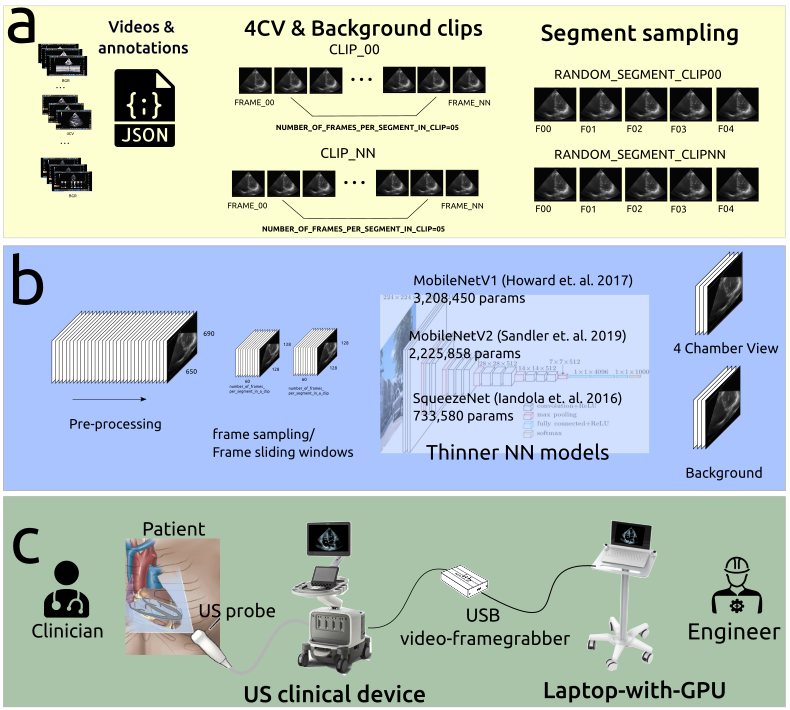
\includegraphics[width=\columnwidth]{../figures/main-figure/versions/drawing-v02}}%%GITHUB
    % {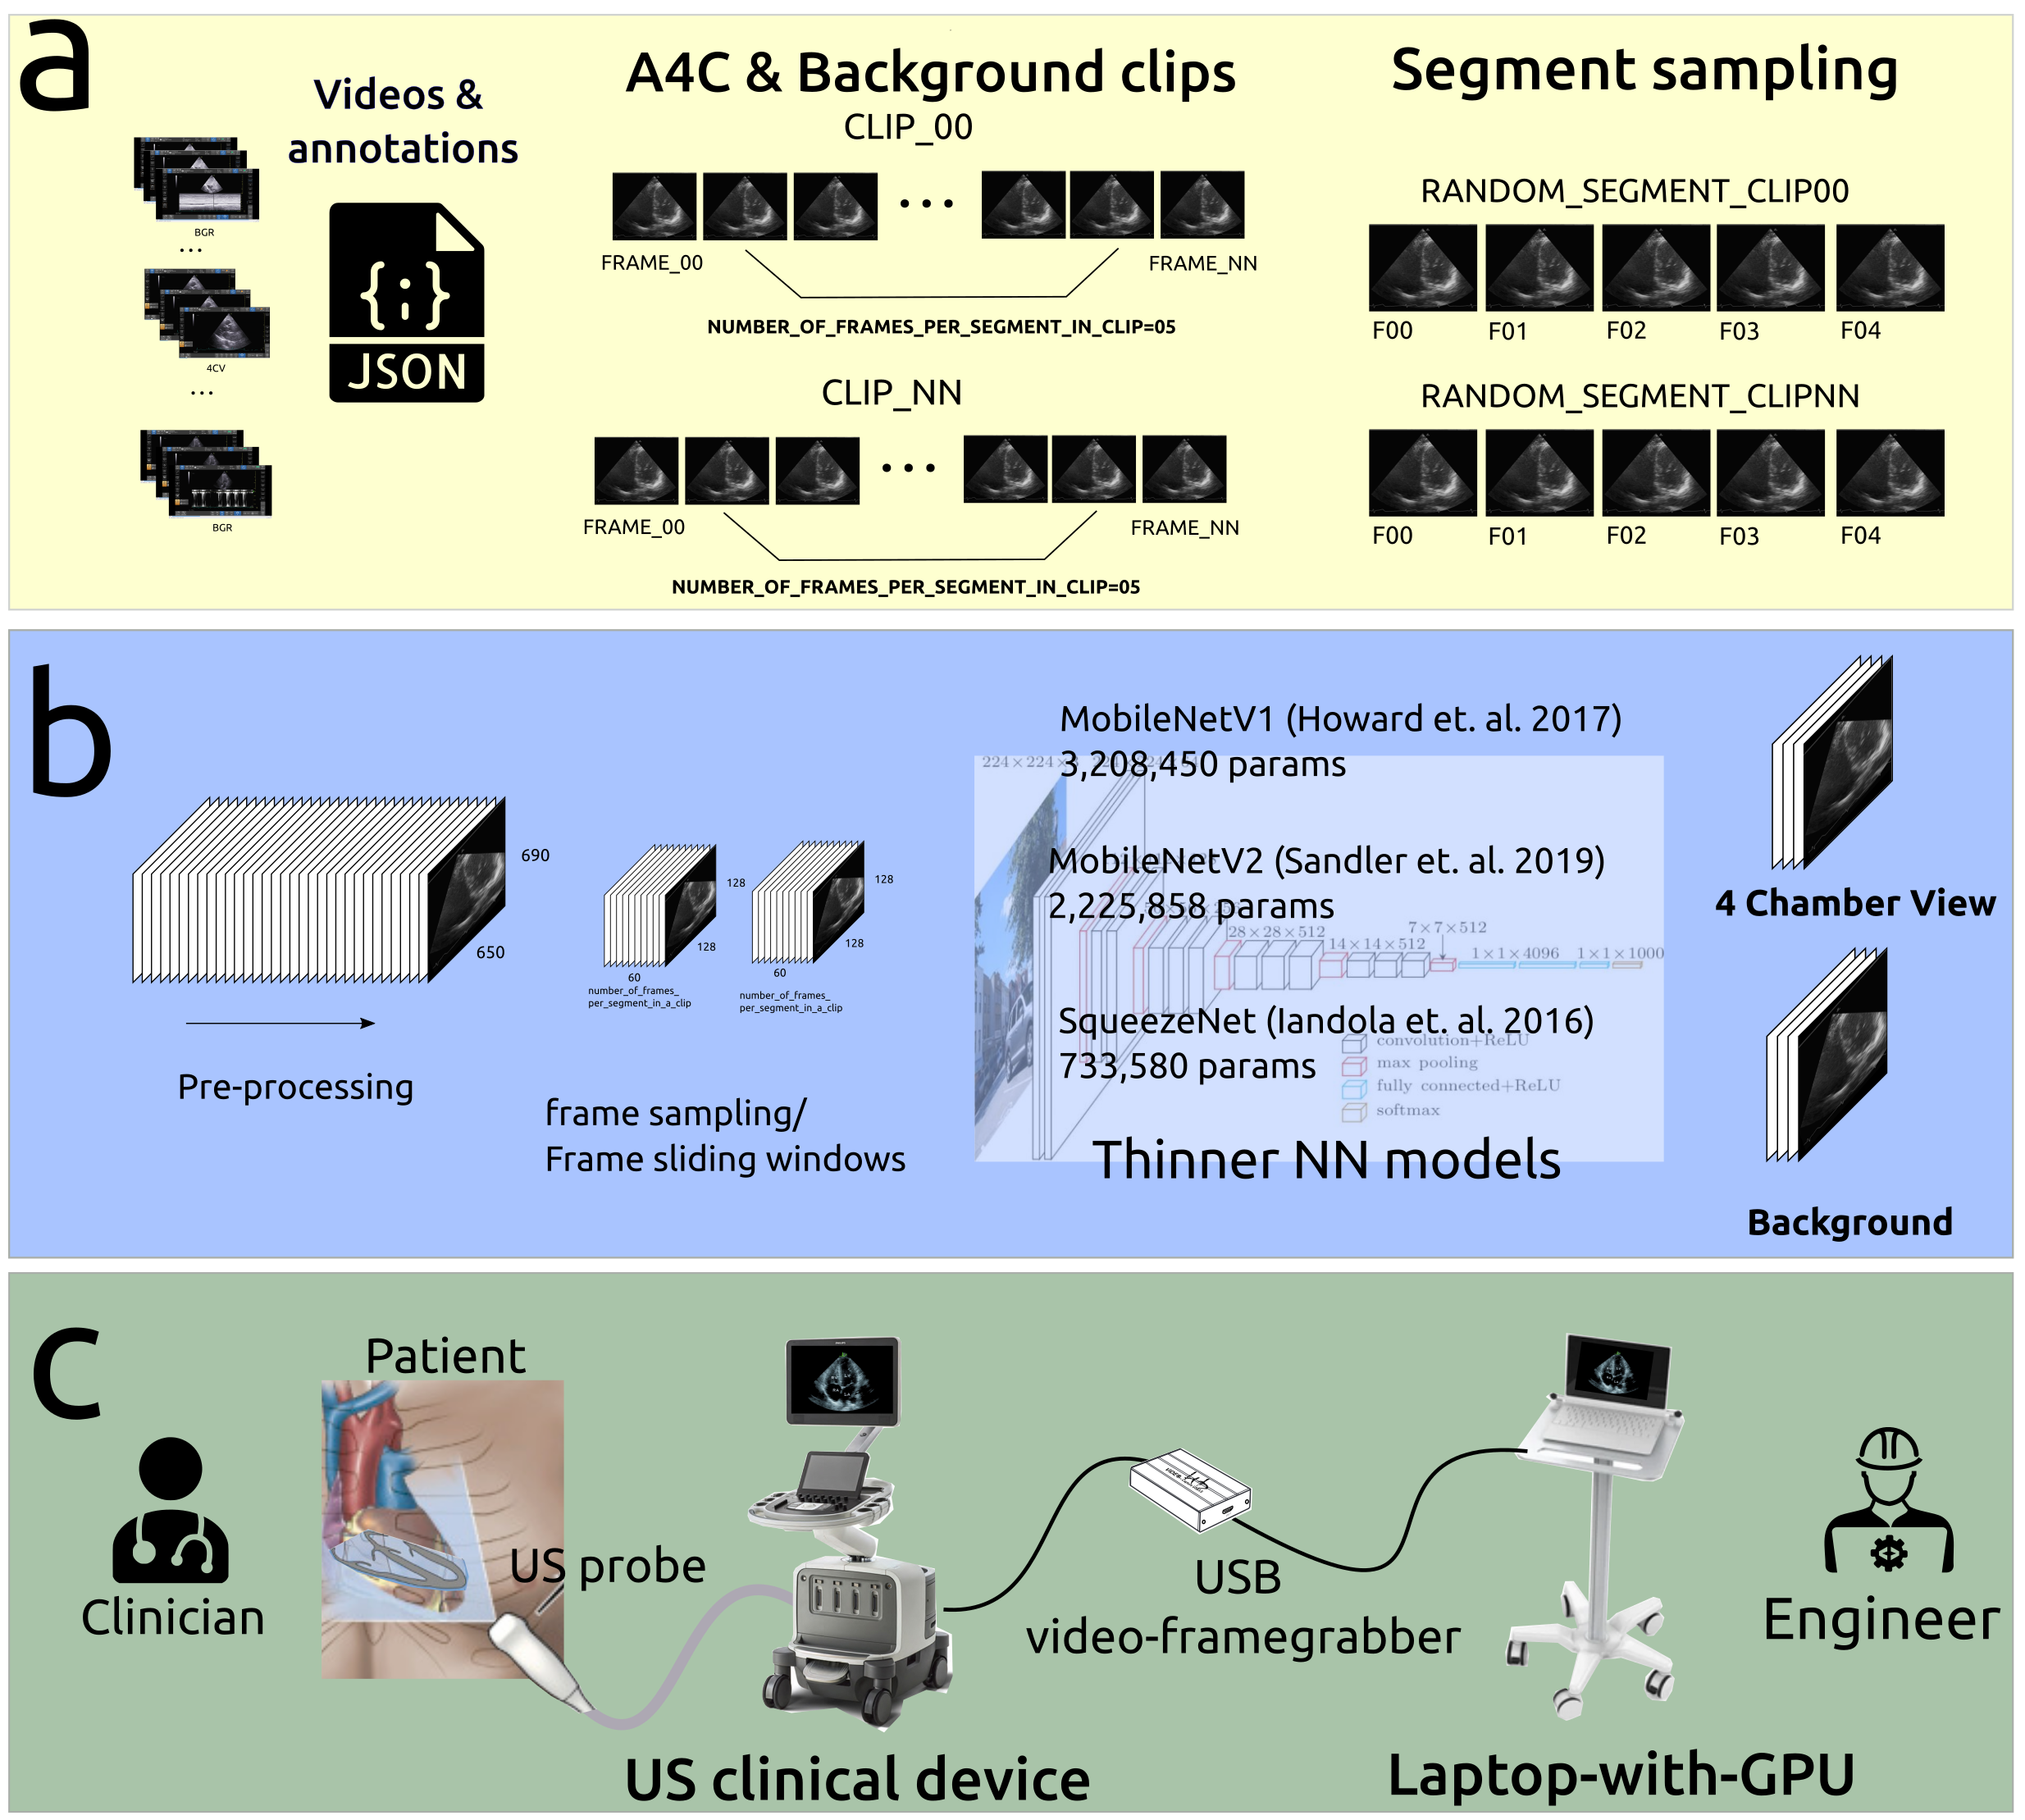
\includegraphics[width=\columnwidth]{figures/main-figure.png}}%%OVERLEAF
    %{\includegraphics[width=\columnwidth]{fig01.png}} %%ARXIV
\end{figure}


\subsubsection{Ethics statement}
This study was approved by the Oxford Tropical Research Ethics Committee (OxTREC) and the HTD Institutional Review Boards (Hospital of Tropical Diseases).
All participants gave written informed consent to participate in the data collection before enrollment.

\subsubsection{Data annotation, validation and management}
Apical 4 Chamber view (A4C) is considered as an important view to compute heart failure measurements from 2D US echocardiography ~\citep{2017_hall_JIntensiveCareSociety}.
For this work, timestamps in the video files for A4C were annotated by one research clinician of 10 years of experience using VGG Image Annotator (VIA).
Then the same clinician  and one researcher validated timestamps annotations where few filenames and timestamps were fixed.
\figureref{fig:main-figure}(a) illustrates video and json files with their A4C and background clips to then be segmented.

\subsection{Model selection and heuristics}
Considering different datasets charactictis (number of frames, clips, pixel image, clinical equipment, etc) and the number of parameters of different networks, we selected four Neural Networks for our ML study:
%VGG-based models~\citep{2015_Simonyan_ICLR},
MobileNetV1~\citep{2017-howared_CoRR_MobileNetV1} with 3,208,450 parameters, MobileNetV2~\citep{Sandler_2018_CVPR_MobileNetV2} with 2,225,858 parameters, and SqueezeNet~\citep{iandola2017squeezenet} with 733,580 parameters.
%complexity of state-of-the-art networks and thinner neural networks,
%and ShrapML \citep{boice2022-in-jimaging} 430,000
%(networks and parameters, respectively).
We then performed heuristics for each model to understand the impact of their performance for different hyperparameters (dataset size, augmentations, frames numbers and clip length).
%as shown in \figureref{fig:heuristics}.
See \appendixref{apd:heuristics} for further details of the heuristics of each model.
%See \figureref{fig:SqueezeNetTrainingResults} for further results on SqueezeNet Training performance.
%\begin{table}[htbp]
%\floatconts
%  {tab:example}%
%  {\caption{Thinner Neural Networks}}%
%{\begin{tabular}{lllll}
%\textbf{Networks} & Parameters \\
%MobileNetV1 \citep{2017-howared_CoRR_MobileNetV1} & 3,208,450    \\
%MobileNetV2 \citep{Sandler_2018_CVPR_MobileNetV2} & 2,225,858   \\
%SqueezeNet \citep{iandola2017squeezenet} & 733,580 \\
%ShrapML \citep{boice2022-in-jimaging} & 430,000
%\end{tabular}}
%\end{table}

\begin{figure}[ht]%htbp
\floatconts
  {fig:heuristics}
  {
      \caption{
          Heuristics for SqueezeNet \citep{iandola2017squeezenet} with dataset of 5 subjects:
          (a) varying batch size and constant number of frames per segment equal to 1, and
          (b) varying number of frames per clip and constant batch size of clips equal to 10.
      }
  }
  {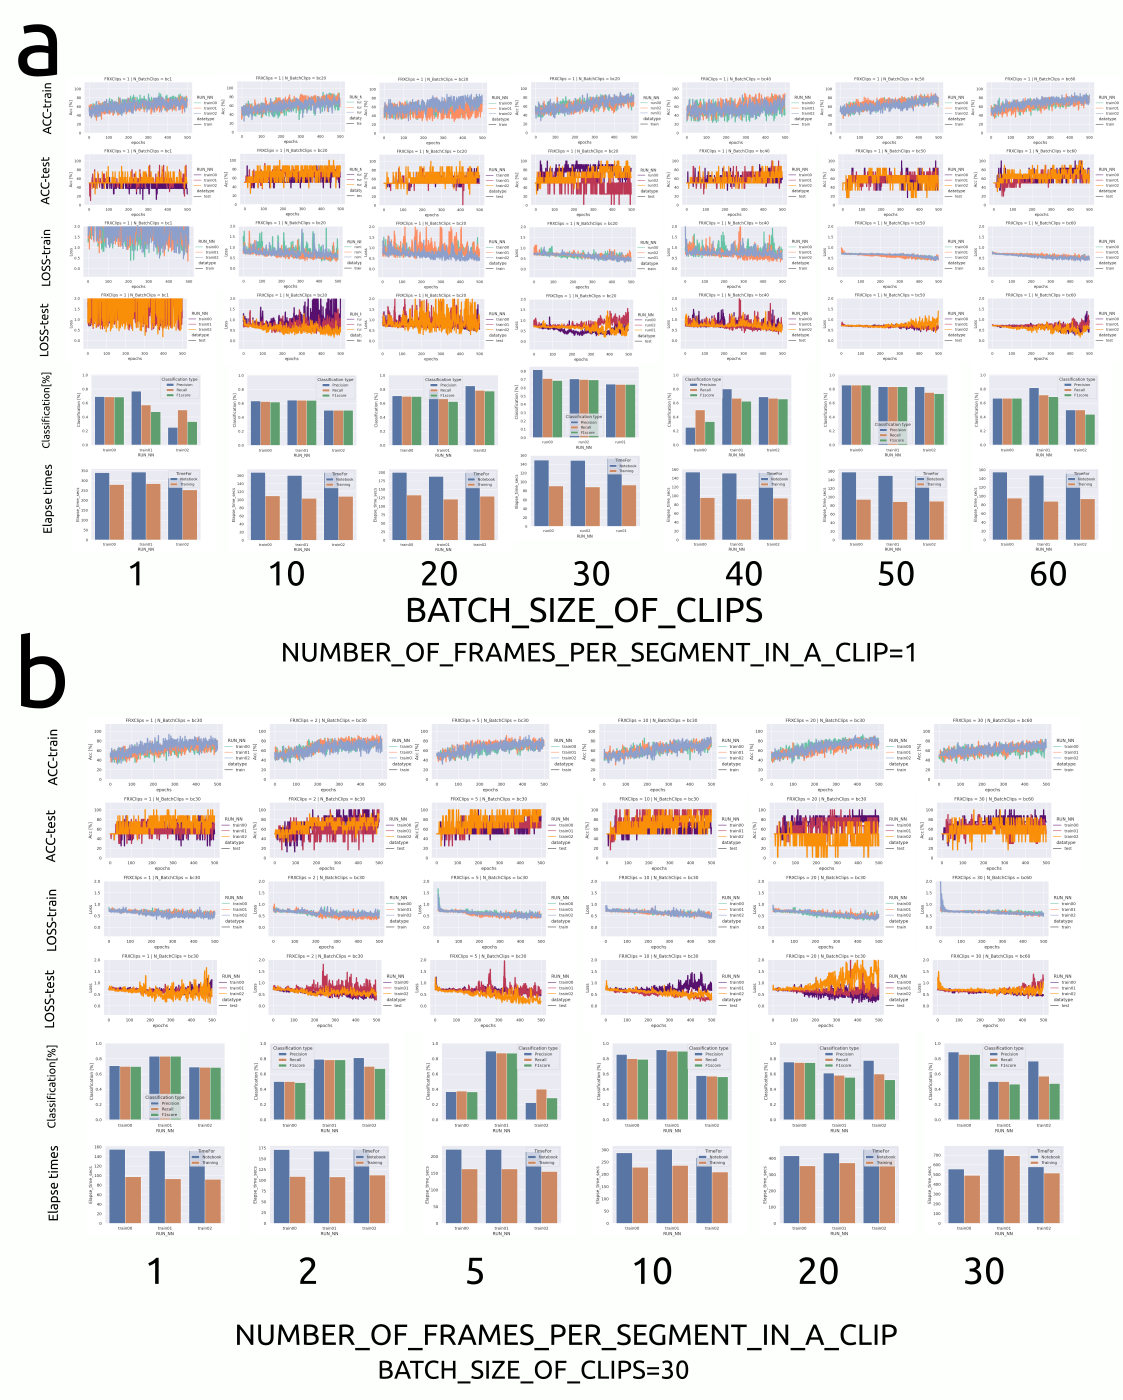
\includegraphics[width=\columnwidth]{../figures/heuristics_results/versions/drawing-v00}}%%GITHUB
    % {\includegraphics[width=\columnwidth]{figures/heuristics.png}}%%OVERLEAF
    %{\includegraphics[width=\columnwidth]{fig01.png}} %%ARXIV
\end{figure}

\section{Conclusions and Future Work}
We presented a machine learning case study, including data selection, validation and management, model selection, validation and in a low-cost clinical system.
For future work, we will investigate real-time inference and deployment of the models, thinner segmentation models and clinical validation in the ICU.
Validation of ML and DL methods for image quality, view classification and segmentation, measurements, detection of abnormalities and diagnosis~\cite{2020_Kusunose_in_CurrentCardiologyReports, 2020_Kusunose_in_Biomolecules, 2021_Kusunose_in_JEchocardiography}.
%Similarly, we are interested in train models with synthetic Ultrasound images for GE Vivid E9, Hitachi Prosound U7, Philips iE 33 Vision, Siemens SC2000, and Toshiba Artida ultrasound systems \citep{brindise2020unsupervised}.
%2D velocity vector fields of flow blow can help to detect abnormal flow patterns as done in fetal and neonatal echocardiography \citep{Meyers2020}.

%\subsection{Real-time AI-empowered echocardiography}
%%In terms of real-time analysis of echocardigraphy
%\subsubsection{State of the art}  \label{subsec:State_of_the_art}
%\citet{woudenberg2018} trained an DenseNet-LSTM with 2000 clips of apical 4 chamber view in which the real-time system made use of 10 input frames and reported a latency of 352.91ms.
%\citet{toussaint2018-MICCAI} proposed ResNet18-SP trained with 85,000 frames of Fetal US imaging, reporting real-time performance at inference time of 40 m$s$ per image ($\sim$20Hz).
%\citet{ostvik2021-TMI} proposed Echo-PWC-Net trained with synthetic, simulated and clinical datasets, reporting real-time performance with 7 frames for the input.
%Recently, \citet{wu2022} applied baselines of UNET with temporal context-aware encoder (TCE) and bidirectional spatiotemporal semantics fusion (BSSF) modules to
%EchoDynamic %datasets
%%(10,030 video sequences with of 200 frames of 112x112 pixes)
%and CAMUS datasets %(450 video with 20 frames of 778x594 pixels)
%, reporting metrics of Dice score (DS), Hausdorff Distance (HD), and area under the curve (AUC).
%To ensure low latency and real-time performance, \citet{wu2022} presented a comparison of eight methods networks including FLOPS (G), number of parameters (M) and speed ($ms/f$) being their method with the lowest speed at 32 $ms/f$ and 56.359 $G$ FLOPS but network size was 74.79M parameters (join motion model with 237.592G FLOPS, 17.315M parameters and seep of 154 $ms/f$).

%\acks{Acknowledgements go here.}


\newpage
\bibliography{../references/references}%%%GITHUB
% \bibliography{references}%%%OVERLEAF
%%%%% SELECT ONE OF THE FOLLOWING COMMANDS %%%%%%%%

%%% TEMPLATE FOR PROCEEDINGS TRACK %%%%
%\documentclass[mlmain,twocolumn]{jmlr}

%% TEMPLATE FOR Extended Abstract Track %%%%%%%
\documentclass[mlabstract,twocolumn]{jmlr}
%\documentclass[mlabstract]{jmlr}

%%%%%%%%%%%%%%%%%%%%%%%%%%%%%%%%%%%%%%%%%%%%%%%%%

%%%%%%%%%%%%%%%%%%%%%%%%
% Watermark
%These 4 commands must be removed for the camera-ready version.
\usepackage[hpos=300px,vpos=70px]{draftwatermark}
\SetWatermarkText{\test}
\SetWatermarkScale{1}
\SetWatermarkAngle{0}
%%%%%%%%%%%%%%%%%%%%%%%%%%


%%OVERLEAF
%% Anyone with this link can edit this project
%% https://www.overleaf.com/4969677577xfsfbjqkrnfx


% The following packages will be automatically loaded:
% amsmath, amssymb, natbib, graphicx, url, algorithm2e


%%% WARNING %%%%
%%% 1) Please, use the packages automatically loaded to manage references, write equations, and include figures and algorithms. The use of different packages could create problems in the generation of the camera-ready version. Please, follow the examples provided in this file.
%%% 2) References must be included in a .bib file.
%%% 3) Write your paper in a single .tex file.
%%%

%%%% SOFTWARE %%%%
%%% Many papers have associated code provided. If that is your case, include a link to the code in the paper as usual and provide a link to the code in the following comment too. We will use the link in the next comment when we generate the proceedings.
%%% Link to code: http://?? (only for camera ready)

 %\usepackage{rotating}% for sideways figures and tables
\usepackage{longtable}% for long tables

 % The booktabs package is used by this sample document
 % (it provides \toprule, \midrule and \bottomrule).
 % Remove the next line if you don't require it.
\usepackage{booktabs}
 % The siunitx package is used by this sample document
 % to align numbers in a column by their decimal point.
 % Remove the next line if you don't require it.
\usepackage[load-configurations=version-1]{siunitx} % newer version
 %\usepackage{siunitx}

 % The following command is just for this sample document:
\newcommand{\cs}[1]{\texttt{\char`\\#1}}

 % Define an unnumbered theorem just for this sample document:
\theorembodyfont{\upshape}
\theoremheaderfont{\scshape}
\theorempostheader{:}
\theoremsep{\newline}
\newtheorem*{note}{Note}

%%%% DON'T CHANGE %%%%%%%%%
\jmlrvolume{}
\firstpageno{1}
\editors{List of editors' names}

\jmlryear{2022}
\jmlrworkshop{Machine Learning for Health (ML4H) 2022}

%\editor{Editor's name}
%%%%%%%%%%%%%%%%%%%%%%%%%%%



\title[Short Title]{
%  Full Title of Article\titlebreak This Title Has A Line Break\titletag{\thanks{sample footnote}}
%Real-time AI-empowered echocardiography for Intensive Care Units in low- and middle-income countries %Mon 20 Jun 11:48:09 BST 2022
%Challenges in Real-time AI-empowered echocardiography for Intensive Care Units in low- and middle-income countries. %Fri 19 Aug 15:36:45 BST 2022
Challenges in Real-time AI-empowered echocardiography for Intensive Care Units in low- and middle-income countries: A Machine Learning Case Study %Fri 19 Aug 16:43:05 BST 2022
}

%%%%%%%%%%%%%%%%%%%%%%%%%%%%%%%%%%%%%
% THE MANUSCRIPT, DATA AND CODE MUST BE ANONYMIZED DURING THE REVIEW PROCESS.
% DON'T INCLUDE ANY INFORMATION ABOUT AUTHORS DURING THE REVIEW PROCESS.
% Information about authors (Full names, emails, affiliations) have to be provided only for the submission of the camera-ready version.  Only in that case, you can uncomment and use the next blocks.
%%%%%%%%%%%%%%%%%%%%%%%%%%%%%%%%%%%%%

   \author{
     \Name{Anonymous Author(s)} \Email{email@sample.com}
      \addr Address
   }

 % Use \Name{Author Name} to specify the name.

 % Spaces are used to separate forenames from the surname so that
 % the surnames can be picked up for the page header and copyright footer.

 % If the surname contains spaces, enclose the surname
 % in braces, e.g. \Name{John {Smith Jones}} similarly
 % if the name has a "von" part, e.g \Name{Jane {de Winter}}.
 % If the first letter in the forenames is a diacritic
 % enclose the diacritic in braces, e.g. \Name{{\'E}louise Smith}

 % *** Make sure there's no spurious space before \nametag ***

 % Two authors with the same address
%   \author{\Name{Author Name1\nametag{\thanks{with a note}}} \Email{abc@sample.com}\and
%   \Name{Author Name2} \Email{xyz@sample.com}\\
%   \addr Address}

  %Three or more authors with the same address:
%   \author{\Name{Author Name1} \Email{an1@sample.com}\\
%   \Name{Author Name2} \Email{an2@sample.com}\\
%   \Name{Author Name3} \Email{an3@sample.com}\\
%   \Name{Author Name4} \Email{an4@sample.com}\\
%   \Name{Author Name5} \Email{an5@sample.com}\\
%   \Name{Author Name6} \Email{an6@sample.com}\\
%   \Name{Author Name7} \Email{an7@sample.com}\\
%   \Name{Author Name8} \Email{an8@sample.com}\\
%   \Name{Author Name9} \Email{an9@sample.com}\\
%   \Name{Author Name10} \Email{an10@sample.com}\\
%   \Name{Author Name11} \Email{an11@sample.com}\\
%   \Name{Author Name12} \Email{an12@sample.com}\\
%   \Name{Author Name13} \Email{an13@sample.com}\\
%   \Name{Author Name14} \Email{an14@sample.com}\\
%   \addr Address}


%%  Authors with different addresses:
%  \author{\Name{Author Name1} \Email{abc@sample.com}\\
%  \addr Address 1
%  \AND
%  \Name{Author Name2} \Email{xyz@sample.com}\\
%  \addr Address 2
% }



\begin{document}

\maketitle

\begin{abstract}
We present a machine learning case study on the current and future challenges of implementing a real-time AI-empowered echocardiography system for ICU in LMICs.
We present reproducible heuristics from a small video dataset of 31 subjects in the ICU, data preparation, curation and labelling, model selection, validation and deployment.
The code and other resources to reproduce this work are available at \url{https://github.com/vital-ultrasound/echocardiography}.
\end{abstract}
\begin{keywords}
deep learning; echocardiography; real-time artificial intelligence;
\end{keywords}

\section{Introduction}
\label{sec:intro}
Echocardiography is an important clinical procedure in Intensive Care Units (ICU) because of the advances of Ultrasound (US) such as portability, low cost, low radiation and its real-time capabilities to access cardiac anatomy \citep{Feigenbaum1996, Vieillard-Baron2008, singh2007, cambell2018}.
Despite that, there various challenges in the current clinical procedures in the ICU:
\begin{itemize}
\setlength\itemsep{0em}
\item Intra-view variability of echocardiograms (physiological variations of subjects and acquisition parameters) and inter-observer variability of expertise for sonographer and radiologist \citep{khamis2017, Feigenbaum1996, field2011},
\item Inter-view similarity of echocardiograms (similar views of valve motion, wall motion, left ventricle, etc) and transducer position during acquisition \citep{zhang2018},
\item Redundant information in the clinical echo system (icons, date, frame rate, etc) \citep{khamis2017} and variation of Ultrasound images from different clinical US systems \citep{brindise2020unsupervised}, and
\item Limited number of expert clinicians to perform US imaging analysis and to provide accurate diagnosis, as well as equipment and hospitalisation requirements in low- and middle-income countries (LMICs) \citep{hao2021-wellcome, 2021-huyNhat-vanHao-in-FAIR-MICCAI}.
\end{itemize}
One promising approach to address such challenges is with the application of Artificial Intelligence to echocardiography.
AI-empowered echocardiography has been successful for detection of different apical views, inter-observer variability of sonographer's expertise, implementation of one-stop AI models with multimodal imaging (US, MRI and clinical data), detection of high risk or low risk of heart failure or automatic detection of endocardial border detection and left ventricle assessment in 2D echocardiography videos \citep{tromp2022, zhang2022-mdpi, behnami2020, ono2022}.
However, there is little to none studies on how real-time AI-empowered echocardiography might impact the ICU in LMICs.
Particularly, how good machine learning practices (data curation, code implementation, model selection, training and tuning; model validation and inference) are addressing challenges on real-time AI-empowered echocardiography in the ICU in LMICs.

This work presents (a) a scoping review of AI-empowered echocardiography for ICU in LMICs and (b) real-time AI-empowered echocardiography, (c) a machine learning case of study of US image classification using deep learning of four chamber views from curated data from LMICs and (d) conclusions future work.
%appendix with further material.

% \subsection{AI-empowered echocardiography}
% Tromp et al. classified a dataset of 1145 2D echocardiography videos as apical 4 chamber (A4C) view, apical 2 chamber (A2C) view, parasternal long axis (PLAX) view, or 2D other views and focused versions of the main views \citep{tromp2022}.
% Authors used CNN of four layers, dense network and softmax output layer, trained with categorical cross-entropy loss function, then a second classifier of an unsupervised deep learning clustering CNN, trained with mean square error and Kullback-Leibler loss functions \citep{tromp2022}.
% %For the remaining dataset (2,126 PSAX-PM echo cines), while the LV segmentation is not available, the ground truth LVEF values are acquired from the patients’ archived information.

% \citet{zhang2022-mdpi}
% reviewed AI's applications in left ventricular systolic function (LVEF) and global longitudinal strain (GLS), pointing out its dependency to the sonographers's expertise (inter-observer variability) and post-processing and variability in different US devices.
% \citet{zhang2022-mdpi} pointed the challenges of AI-enhanced echocargiografy for interpretability of results and its sensitivity to sample shortage, to which authors mention about the potentials of multimodal imaging (us, mri and clinical data) to improve detection rate of diseases.

% \citet{behnami2020} applied DenseNet-like network for feature learning and RNN unit with bidirectional Gated Recurrent Units to alleviate loss of information from the earlier frames of echos to automatically detect high risk or low risk of heart failure with reduced ejection fraction with an overall accuracy of 83.15\%, precision of 82.6\% and recall of 81.1\%.
% \citet{behnami2020} mentioned that EF is highly user-dependant to which they propose to collect more data,

% \citet{liu2021JMIA} proposed pyramid local attention neural network (PLANet) to improve segmentation performance of automatic methods in 2D echocardiography.
% PLANet was evaluated with CAMUS and sub-EchoNet-Dynamic datasets, showing a better performance against geometric and clinical metrics.

% \citet{ulloaCerna2021} made use of DNN to learn spatiotemporal features from echocardiography video data to enhance clinical prediction of 1 yr all-cause mortality where video echo data linked to EHR data that included hand-crafted echocardiography-derived measurements (EDMs), additional clinical variables and individual outcomes.
% The DNN model presents "superior prediction performance" over four cardiologist and two benchmark clinical models: the pooled cohort equations (PCE) and Seattle Heart Failure (SHF) risk score \citep{ulloaCerna2021}.
% \citet{ulloaCerna2021} used "full, raw (annotation-free) echocardiographic videos to make predictions by learning from more than 812,278 clinically acquired echocardiography videos of the heart (50 million images)."

% \citet{jafari2021} pointed out the challenges of obtained high quality for less experience operators and the hight variability or echo quality adn cardiovascular structures across different patients to which authors proposed "Bayesian deep learning approach for fully automatic LVEF estimation based on segmentation of the left ventricle (LV) in parasternal short-axis papillary muscles (PSAX-PM) level".
% \citet{jafari2021} made use of 2,680 patients with PSAX-PM echo cine acquired by a variety of ultrasound devices, namely iE33, Vivid i/7/9/95, Sonosite, and Sequoia (only 554 echo cines were considered as ground truth with LV mask delineated by an experienced level III echocardiographer).

% Ono et al. applied different models where Unet++ demonstrated good performance for automatic endocardial border detection and left ventrical assessment in 2D echocardiography videos \citep{ono2022}.
% The datasets to train networks was made of 2798 images from 118 videos of which 22 videos with 465 frames were for 4CV \citep{ono2022}.
% Ono et al. also touched on the challenges of providing explainable AI for US imaging.


\section{AI-empowered echocardiography for ICU in LMICs}
\citet{hanson2001} reviewed various applications of AI in the ICU where real-time analysis of waveforms of electrocardiograms and electroencephalograms using neural network were used to identify cardiac ischemia and diagnosis myocardial ischemia.
\citet{hanson2001} also reviewed various ICU scenarios where variables such as central venous pressure (CVP), left ventricular ejection fraction (EF), heart rate (HR), hemoglobin (HGB) and oxygen saturation (O2sat) were used with Bayesian networks to provide probabilistic cardiac output.
%\citet{hanson2001} also touched on data visualisation to demonstrate the hypothetical ICU for large number of patients (head injury, sepsis, acute respiratory distress syndrome, etc).
\citet{Ghorbani-DigitalMedicineNature-JAN2020} reported how deep learning models predicts systematic phenotypes which are difficult for human interpreters from echocardiogram images, the extraction of labels local structures and features (e.g. pacemaker lead, dilation of left atrium, hypertrophy for left ventricular) and labels from the physician-interpreted report (e.g, catheters, pacemaker, and defibrillator leads).
%to predict age, sex, weight and height
%and make use of such models
%Authors trained CCN models with 2.6 million echocardiogram images from 2850 patients with
\citet{CHEEMA2021JACCCaseReports} presented five cases covid-19 intensive care unit (ICU) to illustrate "how decision making affect in patient care" and how the use of AI-enabled provided real-time guidance to acquire desired cardiac US with the steering of user's transducer position and hand movement.
Recently, \citet{hong2022} reviewed 673 papers that made use of machine learning to help for clinical decision in the ICU, of these studies the majority used supervised learning (91\%) and few of them applied unsupervised learning and reinforcement learning.
Similarly, \citet{hong2022} identified 20 of the most frequent variables in the ICU, being the top five (age, sex, heart rate, respiratory rate, and pH) in machine learning pipelines.
\citet{hong2022} mentioned that typical outcomes in the ICU are mortality, survival, and long-term quality of life and included typical patient outcomes, specific diseases, and stay of time evaluation and specific diseases where the most studied are sepsis, infection and kidney injury.
%For specific diseases, the most studied are sepsis, infection and kidney injury; and trends with liver diseases and severe cancerl and others like cardica diseases, brain diseases;
However, there is few research on AI-empowered echocardiography for ICU in LMICs where, for instance, \cite{2021-huyNhat-vanHao-in-FAIR-MICCAI} reported challenges in resourced limited ICUs including: infrastructure, education and personnel, data pipelines, regulation and trust in AI.
Also, \cite{2021-kerdegari-Applied-Sciences-MDPI, 2021-kerdegari-ISBI-IEEE, 2021-huyNhat-kerdegari-in-FAIR-MICCAI} presented a deep-learning lung US pathology classifier for ICU patient in LMIC, stating the challenges of data imbalance, integration of technology and IT infrastructure of the ICU in LMIC.

\section{Real-time AI-empowwered echocardiography}
%In terms of real-time analysis of echocardigraphy, , 
\citet{woudenberg2018} trained an DenseNet-LSTM with 2K clips of 4 chamber view in which the real-time system made use of 10 input frames and reported a latency of 352.91ms.
\citet{toussaint2018-MICCAI} proposed ResNet18-SP trained with 85k frames of Fetal US imaging, reporting real-time performance at inference time of 40 m$s$ per image or $\sim$20Hz.
\citet{ostvik2021-TMI} proposed Echo-PWC-Net trained with Synthetic/Simulated/Clinical, reporting real-time performance with 7 frames for the input.
Recently, \citet{wu2022} applied baselines of UNET with temporal context-aware encoder (TCE) and bidirectional spatiotemporal semantics fusion (BSSF) modules to EchoDynamic datasets (10030 video sequences with of 200 frames of 112x112 pixes) and CAMUS datasets  (450 video with 20 frames of 778x594 pixels), reporting metrics of Dice score (DS), Hausdorff Distance (HD), and area under the curve (AUC).
Similarly, \citet{wu2022} presented speed analysis to ensure low latency and real-time performance for eight methods using calculations number FLOPS (G), number of parameters (M) and speed ($ms/f$).
%which lowest one was 32 $ms/f$.

\subsection{Classification of echochardiograms}
\citet{khamis2017} considered 309 clinical echocardiogram of apical views which were visually classified and labelled by two experts into three classes: 103 a2c views, 103 a4c views and 103 alx views to then applied spatio-temporal feature extraction (Cuboic Detector) and supervised learning dictionary (LC-KSVD) resulting in an overall recognition rate of 95\%.
\citet{woudenberg2018} applied DenseNet and LSTM to extract temporal information on sequences of 16K echo cine frames to classify 14 heart views with an average accuracy of 92.35\%.
%\citet{woudenberg2018} implemented a Tensorflow runner that performs contrast enhancement to then sent each frame to three identical CNNs running in separated threads to prevent lag during inference times.
%Then a shared buffer collects extracted features from CNNs to then awake the thread for the LSTM network from the previous ten frames to produce classification and quality prediction.
\citet{woudenberg2018} also presents timing diagrams to quantify frame arrival and real-time performance to operate at 30 frames per second, while providing feedback with a mean latency of 352.91 ± 38.27 m$s$ when measured from the middle of the ten-frame sequence.
\citet{zhang2018} performed view classification with 277 echocardiograms to create a 23-class models (including a4c no occlusions, a4c occluded LA, a4c occluded LV, etc) using 13-layer CNN with 5-fold cross-validation for accuracy assessment and resulting in 84\% for overall accuracy where challenges for partial obscured LVs for a2c, a3c and a4c.
Similarly, \citet{zhang2018} applied U-net to segment 5 views (a2c, a3c, a4c, PSAX, PLAX) and CNN model for 3 cardiac diseases with the use of A4c capturing most of the information for the diseases.

\subsection{Thinner neural networks to classify US images} \label{subsec:thinnerNets}
\citet{baumgartner2017-IEEETransMedImag} proposed SonoNet which is a VGG-based architecture, having the same first 13 layers of VGG16, and SmallNet, loosely inspired by AlexNet, for real-time detection and bounding box localisation of standard views in freehand fetal US.
\citet{toussaint2018-MICCAI} applied four feature extraction networks couple with batchnormalization and soft proposal layer (VGG13-SP, VGG16-SP, ResNet18-SP, ResNet34-SP), resulting in 0.912 of average accuracy over six classes of fetal US views with ResNet18-SP.
\citet{Al-Dhabyani2019-IJACSA} applied AlexNet and transfer learning of four architectures (VGG16, Inception, ResNet, and NASNet) without augmentation and with three augmentation techniques to perform tumor classification of breast ultrasound imaging.
Authors stated that transfer learning with NASNet presented the best accuracy with 99\% using BUSI+B datasets with DAGAN augmentation.
\citet{xie2020-physics-in-medicine-biology} proposed a dual-sampling convolutional neural network (DSCNN) for US image breast cancer classification, being DSCNN more efficient than AlexNet, VGG16, ResNet18, GoogleNet and EfficientNet.
Recently, \citet{snider2022-ScientificReports} reported summaries of CNN heuristics to detect shrapnel in US images, including layer activators, 2D CNN layer architectures, model optimisers dense nodes, and the effect of image augmentation and dropout rate and epoch number.
Similarly, \citet{boice2022-in-jimaging} proposed ShrapML, a CNN model to detect shrapnel in US imaging.
Authors compared ShrapML (8layers--6CNN,2FC, 0.43 million of parameters) against DarkNet19, GoogleNet, MobileNetv2 and SqueezeNet, being ShrapML 10x faster than MobileNet2 which offered the highest accuracy.

\section{Machine learning case study}

\subsection{Dataset}
Echocardiography videos of 31 subjects in the ICU were considered for this work which were collected by four radiologists using the clinical devices: GE Venue Go machine and GE convex probe C1-5-D.
The 31 subjects has the following demographics:
Sex: \% (Male): 58.1\%;
Age: mean, years (std): 38.70 (16.08);
Weight: mean, Kg (std): 61.51 (15.06);
Height: mean, m (std): 1.62 (0.07);
BMI: mean (std): 23.80 (4.30);
Sepsis \% (with): 61.3\%;
Dengue \% (with): 54.8\%, and
Tetanus \% (with): 87.1\%.
See \appendixref{apd:datasets} for further details on the demographics of the dataset, including the complete dataset of 87 subjects.

\subsubsection{Ethics statement}
This study was approved by the Oxford Tropical Research Ethics Committee (OxTREC) and the HTD Institutional Review Boards (Hospital of Tropical Diseases).
All participants gave written informed consent to participate before enrollment.

\subsubsection{Data annotation, validation and management}
Timestamps of 4 chamber views of video files from 31 subjects were annotated by one research clinician of 10 years of experience using VGG Image Annotator (VIA).
Then the same clinician  and one researcher validated annotations in a round of two iterations where few filenames timestamps were fixed.

\subsection{Model selection and heuristics}
Considering \sectionref{subsec:thinnerNets}, we selected four thinner Neural Networks for our ML study: MobileNetV1 \citep{2017-howared_CoRR_MobileNetV1} 3,208,450; MobileNetV2 \citep{Sandler_2018_CVPR_MobileNetV2} 2,225,858; SqueezeNet \citep{iandola2017squeezenet} 733,580 and ShrapML \citep{boice2022-in-jimaging} 430,000 (networks and parameters, respectively).
We then performed heuristics for each model to understand their performance for different hyperparameters (datasize, augmentations and clip length) as shown in \figureref{fig:heuristics}.
See \appendixref{apd:heuristics} for further details on each model.
%See \figureref{fig:SqueezeNetTrainingResults} for further results on SqueezeNet Training performance.
%\begin{table}[htbp]
%\floatconts
%  {tab:example}%
%  {\caption{Thinner Neural Networks}}%
%{\begin{tabular}{lllll}
%\textbf{Networks} & Parameters \\
%MobileNetV1 \citep{2017-howared_CoRR_MobileNetV1} & 3,208,450    \\
%MobileNetV2 \citep{Sandler_2018_CVPR_MobileNetV2} & 2,225,858   \\
%SqueezeNet \citep{iandola2017squeezenet} & 733,580 \\
%ShrapML \citep{boice2022-in-jimaging} & 430,000
%\end{tabular}}
%\end{table}
\begin{figure}[htbp]
\floatconts
  {fig:main-figure}
  {\caption{
      Proposed low-cost clinical system for real-time AI-empowered echocardiography:
      (a) deep-learning pipeline with thinner NNs, and
      (b) clinical system: Epiq Q7, cardiac probe X5-1, USB video-frame grabber and 16GB GeForce RTX 3080 GPU Laptop
    }
  }
  {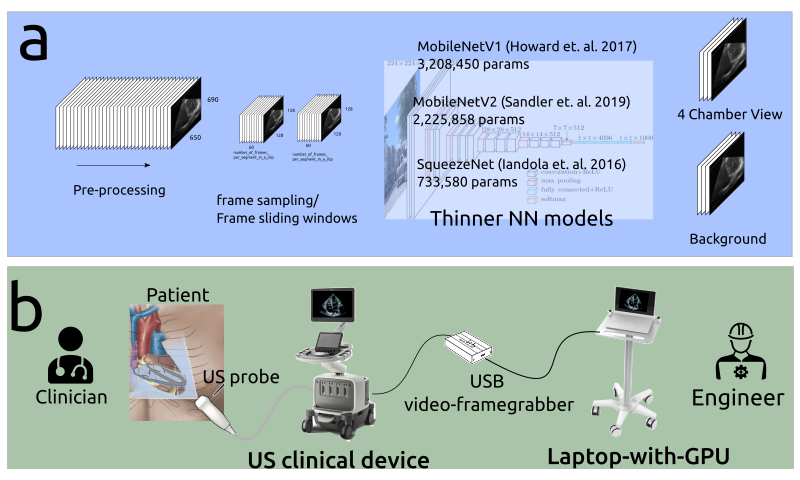
\includegraphics[width=\columnwidth]{../figures/main-figure/versions/drawing-v01}}%%GITHUB
    % {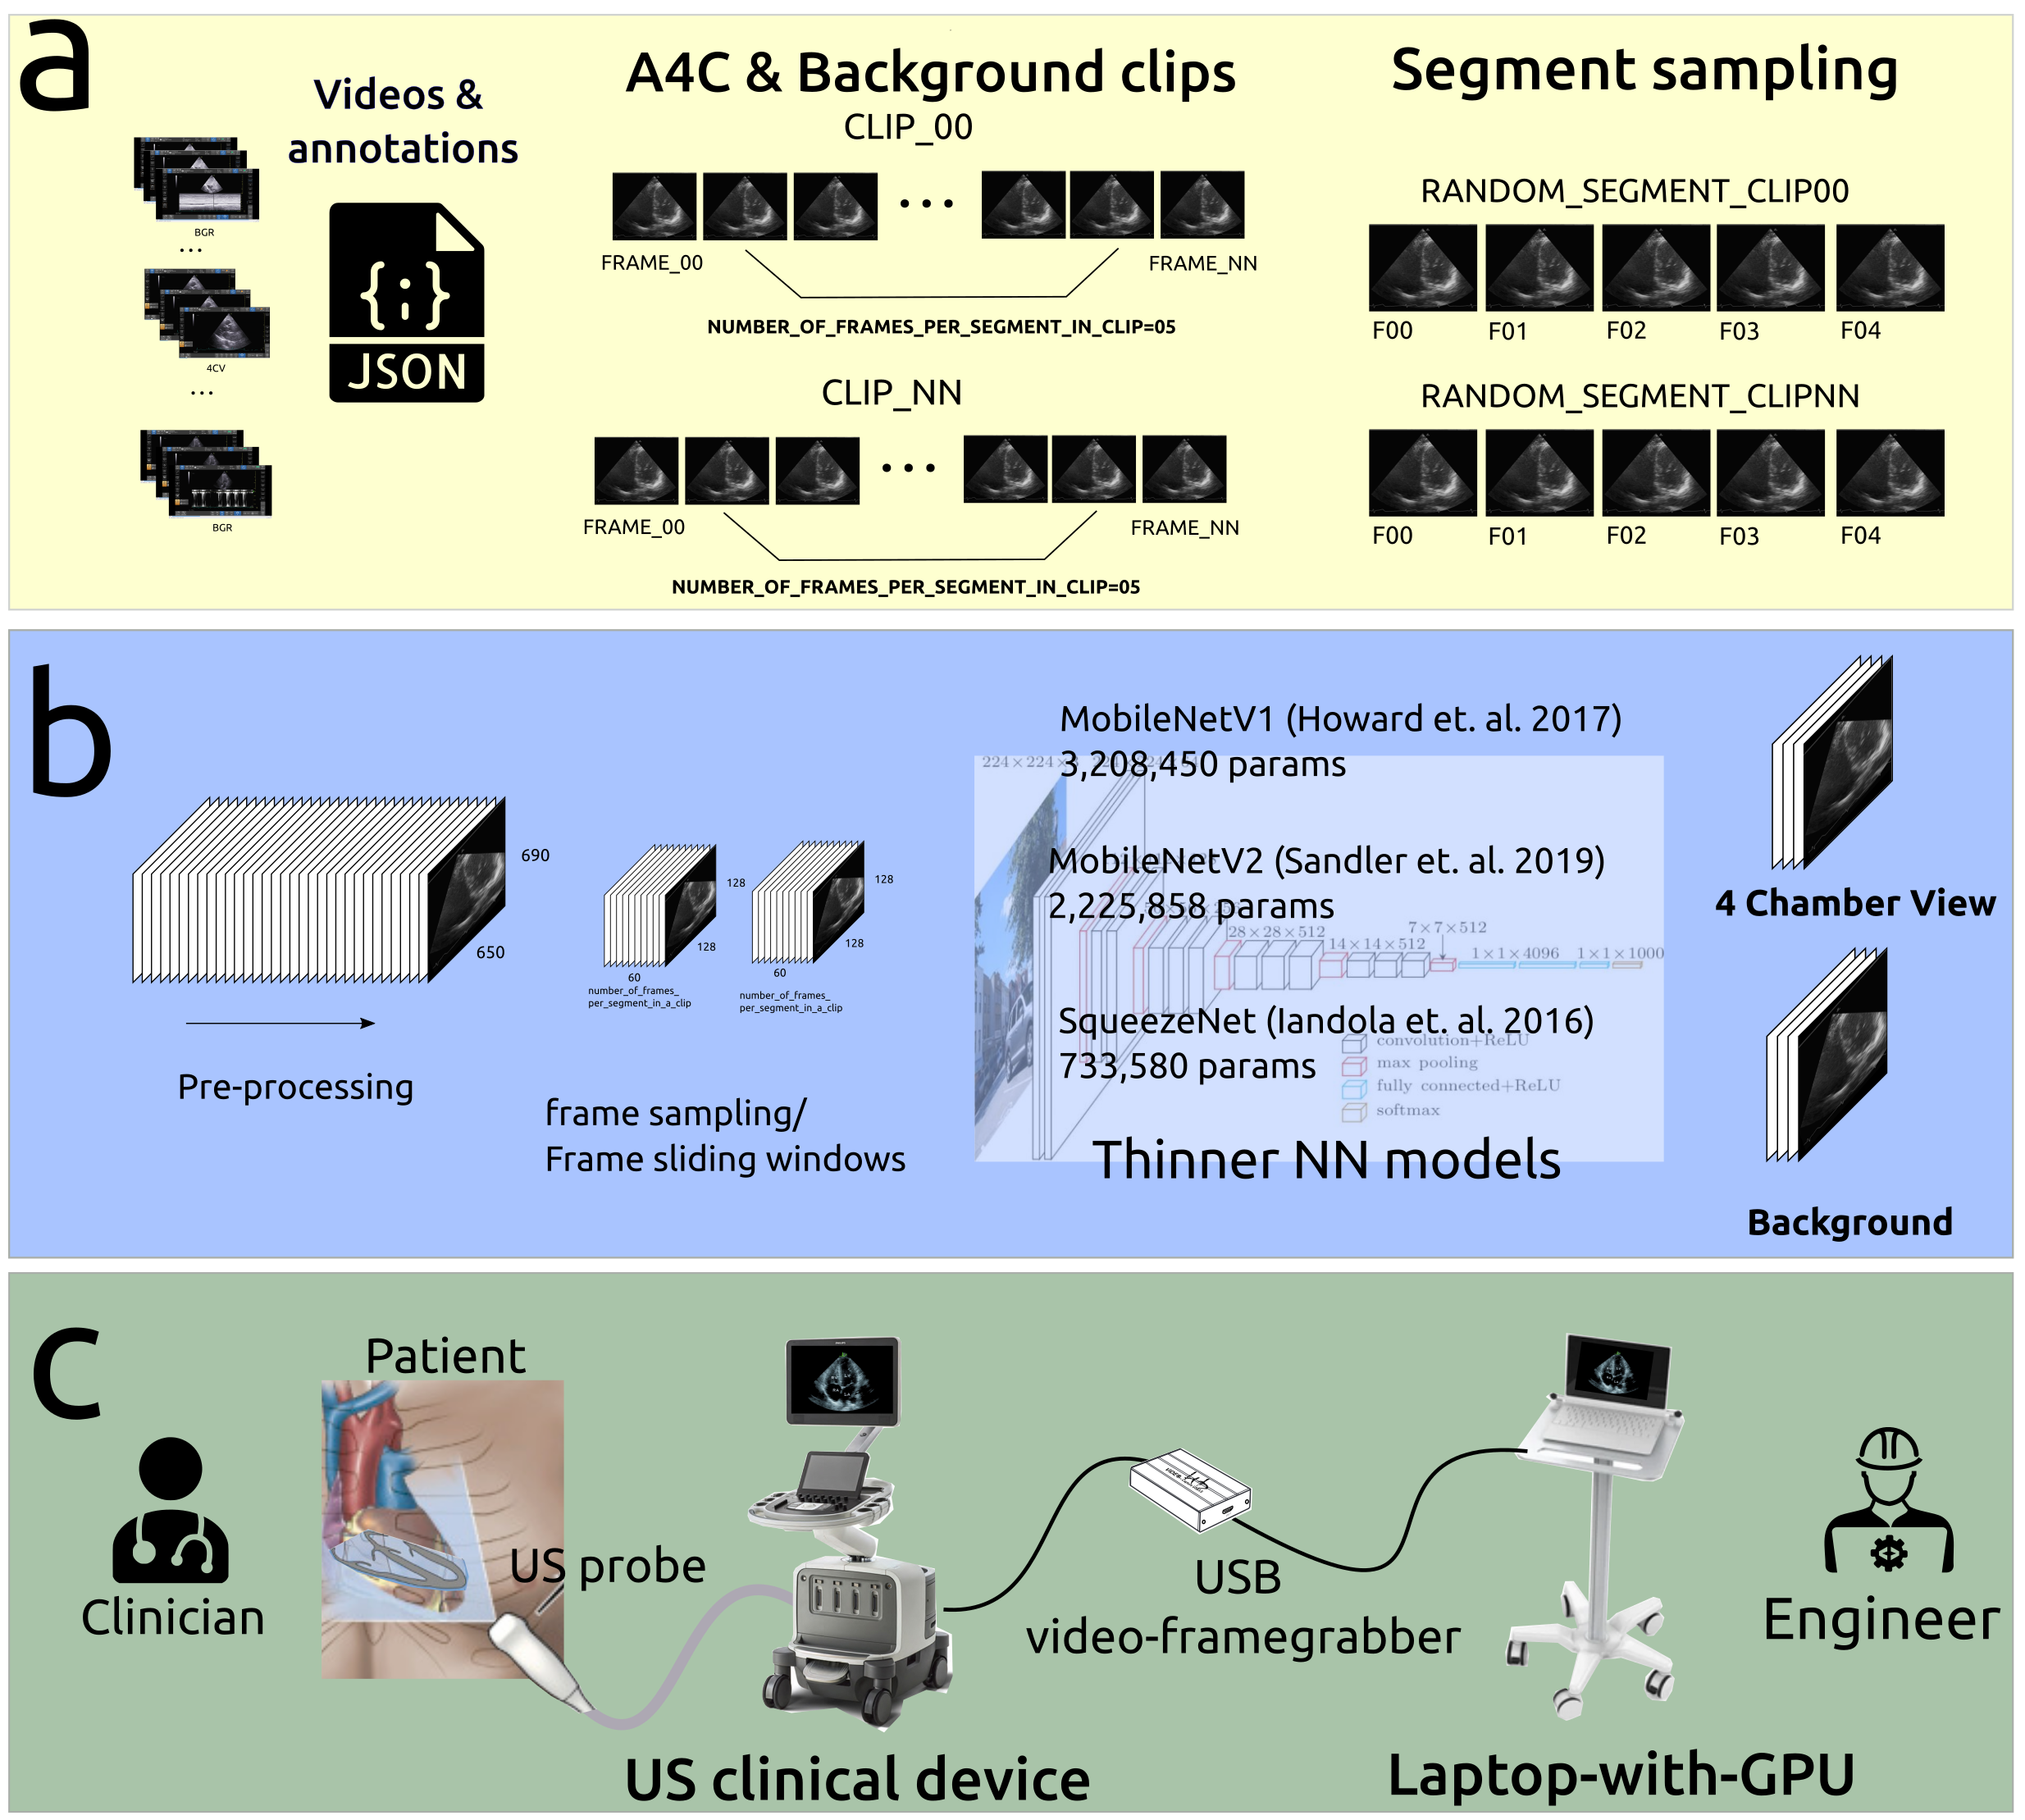
\includegraphics[width=\columnwidth]{figures/main-figure.png}}%%OVERLEAF
    %{\includegraphics[width=\columnwidth]{fig01.png}} %%ARXIV
\end{figure}

\begin{figure}[htbp]
\floatconts
  {fig:heuristics}
  {
      \caption{
          Heuristics for SqueezeNet \citep{iandola2017squeezenet} with dataset of 5 subjects:
          (a) varing batch size and constant number of frames per segment equal to 1, and
          (b) varing number of frames per clip and constant batch size of clips equal to 10.
      }
  }
  {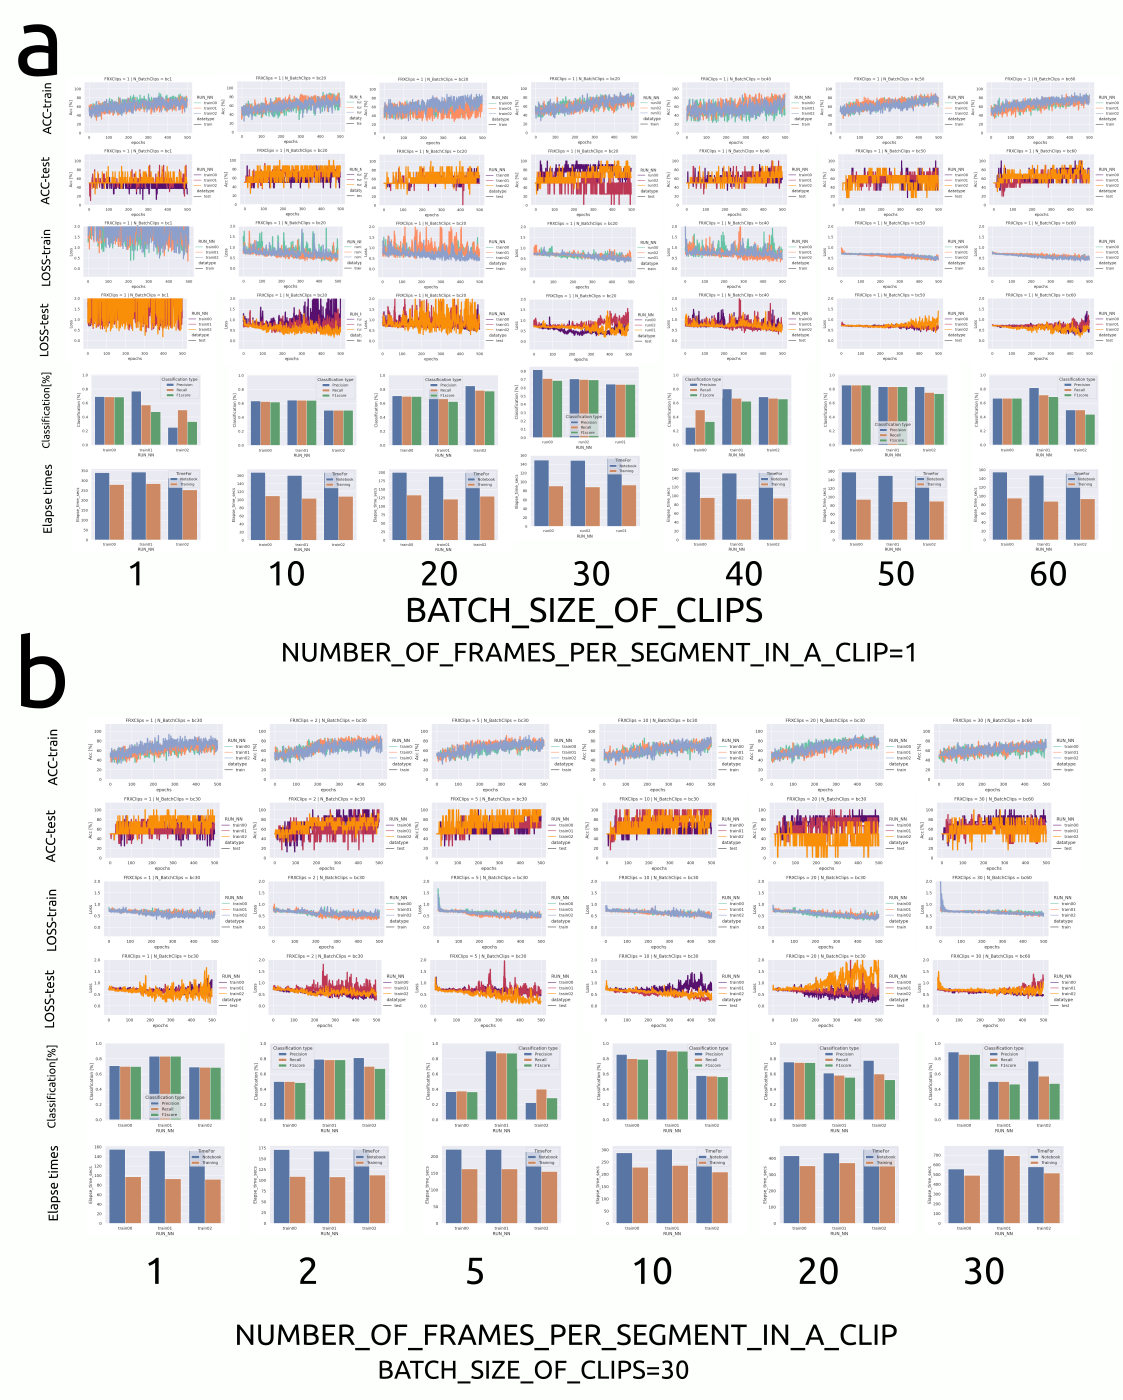
\includegraphics[width=\columnwidth]{../figures/heuristics_results/versions/drawing-v00}}%%GITHUB
    % {\includegraphics[width=\columnwidth]{figures/heuristics.png}}%%OVERLEAF
    %{\includegraphics[width=\columnwidth]{fig01.png}} %%ARXIV
\end{figure}

\section{Conclusions and Future Work}
We presented a machine learning case study, including data selection, validation and management, model selection, validation and low-cost clinical system.
Future work, we will investigate thinner segmentation models, model deployment and clinical validation in the ICU.
%Similarly, we are interested in train models with synthetic Ultrasound images for GE Vivid E9, Hitachi Prosound U7, Philips iE 33 Vision, Siemens SC2000, and Toshiba Artida ultrasound systems \citep{brindise2020unsupervised}.
%2D velocity vector fields of flow blow can help to detect abnormal flow patterns as done in fetal and neonatal echocardiography \citep{Meyers2020}.

%\acks{Acknowledgements go here.}

\bibliography{../references/references}%%%GITHUB
% \bibliography{references}%%%OVERLEAF
%%%%% SELECT ONE OF THE FOLLOWING COMMANDS %%%%%%%%

%%% TEMPLATE FOR PROCEEDINGS TRACK %%%%
%\documentclass[mlmain,twocolumn]{jmlr}

%% TEMPLATE FOR Extended Abstract Track %%%%%%%
\documentclass[mlabstract,twocolumn]{jmlr}
%\documentclass[mlabstract]{jmlr}

%%%%%%%%%%%%%%%%%%%%%%%%%%%%%%%%%%%%%%%%%%%%%%%%%

%%%%%%%%%%%%%%%%%%%%%%%%
% Watermark
%These 4 commands must be removed for the camera-ready version.
\usepackage[hpos=300px,vpos=70px]{draftwatermark}
\SetWatermarkText{\test}
\SetWatermarkScale{1}
\SetWatermarkAngle{0}
%%%%%%%%%%%%%%%%%%%%%%%%%%


%%OVERLEAF
%% Anyone with this link can edit this project
%% https://www.overleaf.com/4969677577xfsfbjqkrnfx


% The following packages will be automatically loaded:
% amsmath, amssymb, natbib, graphicx, url, algorithm2e


%%% WARNING %%%%
%%% 1) Please, use the packages automatically loaded to manage references, write equations, and include figures and algorithms. The use of different packages could create problems in the generation of the camera-ready version. Please, follow the examples provided in this file.
%%% 2) References must be included in a .bib file.
%%% 3) Write your paper in a single .tex file.
%%%

%%%% SOFTWARE %%%%
%%% Many papers have associated code provided. If that is your case, include a link to the code in the paper as usual and provide a link to the code in the following comment too. We will use the link in the next comment when we generate the proceedings.
%%% Link to code: http://?? (only for camera ready)

 %\usepackage{rotating}% for sideways figures and tables
\usepackage{longtable}% for long tables

 % The booktabs package is used by this sample document
 % (it provides \toprule, \midrule and \bottomrule).
 % Remove the next line if you don't require it.
\usepackage{booktabs}
 % The siunitx package is used by this sample document
 % to align numbers in a column by their decimal point.
 % Remove the next line if you don't require it.
\usepackage[load-configurations=version-1]{siunitx} % newer version
 %\usepackage{siunitx}

 % The following command is just for this sample document:
\newcommand{\cs}[1]{\texttt{\char`\\#1}}

 % Define an unnumbered theorem just for this sample document:
\theorembodyfont{\upshape}
\theoremheaderfont{\scshape}
\theorempostheader{:}
\theoremsep{\newline}
\newtheorem*{note}{Note}

%%%% DON'T CHANGE %%%%%%%%%
\jmlrvolume{}
\firstpageno{1}
\editors{List of editors' names}

\jmlryear{2022}
\jmlrworkshop{Machine Learning for Health (ML4H) 2022}

%\editor{Editor's name}
%%%%%%%%%%%%%%%%%%%%%%%%%%%



\title[Short Title]{
%  Full Title of Article\titlebreak This Title Has A Line Break\titletag{\thanks{sample footnote}}
%Real-time AI-empowered echocardiography for Intensive Care Units in low- and middle-income countries %Mon 20 Jun 11:48:09 BST 2022
%Challenges in Real-time AI-empowered echocardiography for Intensive Care Units in low- and middle-income countries. %Fri 19 Aug 15:36:45 BST 2022
Challenges in Real-time AI-empowered echocardiography for Intensive Care Units in low- and middle-income countries: A Machine Learning Case Study %Fri 19 Aug 16:43:05 BST 2022
}

%%%%%%%%%%%%%%%%%%%%%%%%%%%%%%%%%%%%%
% THE MANUSCRIPT, DATA AND CODE MUST BE ANONYMIZED DURING THE REVIEW PROCESS.
% DON'T INCLUDE ANY INFORMATION ABOUT AUTHORS DURING THE REVIEW PROCESS.
% Information about authors (Full names, emails, affiliations) have to be provided only for the submission of the camera-ready version.  Only in that case, you can uncomment and use the next blocks.
%%%%%%%%%%%%%%%%%%%%%%%%%%%%%%%%%%%%%

   \author{
     \Name{Anonymous Author(s)} \Email{email@sample.com}
      \addr Address
   }

 % Use \Name{Author Name} to specify the name.

 % Spaces are used to separate forenames from the surname so that
 % the surnames can be picked up for the page header and copyright footer.

 % If the surname contains spaces, enclose the surname
 % in braces, e.g. \Name{John {Smith Jones}} similarly
 % if the name has a "von" part, e.g \Name{Jane {de Winter}}.
 % If the first letter in the forenames is a diacritic
 % enclose the diacritic in braces, e.g. \Name{{\'E}louise Smith}

 % *** Make sure there's no spurious space before \nametag ***

 % Two authors with the same address
%   \author{\Name{Author Name1\nametag{\thanks{with a note}}} \Email{abc@sample.com}\and
%   \Name{Author Name2} \Email{xyz@sample.com}\\
%   \addr Address}

  %Three or more authors with the same address:
%   \author{\Name{Author Name1} \Email{an1@sample.com}\\
%   \Name{Author Name2} \Email{an2@sample.com}\\
%   \Name{Author Name3} \Email{an3@sample.com}\\
%   \Name{Author Name4} \Email{an4@sample.com}\\
%   \Name{Author Name5} \Email{an5@sample.com}\\
%   \Name{Author Name6} \Email{an6@sample.com}\\
%   \Name{Author Name7} \Email{an7@sample.com}\\
%   \Name{Author Name8} \Email{an8@sample.com}\\
%   \Name{Author Name9} \Email{an9@sample.com}\\
%   \Name{Author Name10} \Email{an10@sample.com}\\
%   \Name{Author Name11} \Email{an11@sample.com}\\
%   \Name{Author Name12} \Email{an12@sample.com}\\
%   \Name{Author Name13} \Email{an13@sample.com}\\
%   \Name{Author Name14} \Email{an14@sample.com}\\
%   \addr Address}


%%  Authors with different addresses:
%  \author{\Name{Author Name1} \Email{abc@sample.com}\\
%  \addr Address 1
%  \AND
%  \Name{Author Name2} \Email{xyz@sample.com}\\
%  \addr Address 2
% }



\begin{document}

\maketitle

\begin{abstract}
We present a machine learning case study on the current and future challenges of implementing a real-time AI-empowered echocardiography system for ICU in LMICs.
We present reproducible heuristics from a small video dataset of 31 subjects in the ICU, data preparation, curation and labelling, model selection, validation and deployment.
The code and other resources to reproduce this work are available at \url{https://github.com/vital-ultrasound/echocardiography}.
\end{abstract}
\begin{keywords}
deep learning; echocardiography; real-time artificial intelligence;
\end{keywords}

\section{Introduction}
\label{sec:intro}
Echocardiography is an important clinical procedure in Intensive Care Units (ICU) because of the advances of Ultrasound (US) such as portability, low cost, low radiation and its real-time capabilities to access cardiac anatomy \citep{Feigenbaum1996, Vieillard-Baron2008, singh2007, cambell2018}.
Despite that, there various challenges in the current clinical procedures in the ICU:
\begin{itemize}
\setlength\itemsep{0em}
\item Intra-view variability of echocardiograms (physiological variations of subjects and acquisition parameters) and inter-observer variability of expertise for sonographer and radiologist \citep{khamis2017, Feigenbaum1996, field2011},
\item Inter-view similarity of echocardiograms (similar views of valve motion, wall motion, left ventricle, etc) and transducer position during acquisition \citep{zhang2018},
\item Redundant information in the clinical echo system (icons, date, frame rate, etc) \citep{khamis2017} and variation of Ultrasound images from different clinical US systems \citep{brindise2020unsupervised}, and
\item Limited number of expert clinicians to perform US imaging analysis and to provide accurate diagnosis, as well as equipment and hospitalisation requirements in low- and middle-income countries (LMICs) \citep{hao2021-wellcome, 2021-huyNhat-vanHao-in-FAIR-MICCAI}.
\end{itemize}
One promising approach to address such challenges is with the application of Artificial Intelligence to echocardiography.
AI-empowered echocardiography has been successful for detection of different apical views, inter-observer variability of sonographer's expertise, implementation of one-stop AI models with multimodal imaging (US, MRI and clinical data), detection of high risk or low risk of heart failure or automatic detection of endocardial border detection and left ventricle assessment in 2D echocardiography videos \citep{tromp2022, zhang2022-mdpi, behnami2020, ono2022}.
However, there is little to none studies on how real-time AI-empowered echocardiography might impact the ICU in LMICs.
Particularly, how good machine learning practices (data curation, code implementation, model selection, training and tuning; model validation and inference) are addressing challenges on real-time AI-empowered echocardiography in the ICU in LMICs.

This work presents (a) a scoping review of AI-empowered echocardiography for ICU in LMICs and (b) real-time AI-empowered echocardiography, (c) a machine learning case of study of US image classification using deep learning of four chamber views from curated data from LMICs and (d) conclusions future work.
%appendix with further material.

% \subsection{AI-empowered echocardiography}
% Tromp et al. classified a dataset of 1145 2D echocardiography videos as apical 4 chamber (A4C) view, apical 2 chamber (A2C) view, parasternal long axis (PLAX) view, or 2D other views and focused versions of the main views \citep{tromp2022}.
% Authors used CNN of four layers, dense network and softmax output layer, trained with categorical cross-entropy loss function, then a second classifier of an unsupervised deep learning clustering CNN, trained with mean square error and Kullback-Leibler loss functions \citep{tromp2022}.
% %For the remaining dataset (2,126 PSAX-PM echo cines), while the LV segmentation is not available, the ground truth LVEF values are acquired from the patients’ archived information.

% \citet{zhang2022-mdpi}
% reviewed AI's applications in left ventricular systolic function (LVEF) and global longitudinal strain (GLS), pointing out its dependency to the sonographers's expertise (inter-observer variability) and post-processing and variability in different US devices.
% \citet{zhang2022-mdpi} pointed the challenges of AI-enhanced echocargiografy for interpretability of results and its sensitivity to sample shortage, to which authors mention about the potentials of multimodal imaging (us, mri and clinical data) to improve detection rate of diseases.

% \citet{behnami2020} applied DenseNet-like network for feature learning and RNN unit with bidirectional Gated Recurrent Units to alleviate loss of information from the earlier frames of echos to automatically detect high risk or low risk of heart failure with reduced ejection fraction with an overall accuracy of 83.15\%, precision of 82.6\% and recall of 81.1\%.
% \citet{behnami2020} mentioned that EF is highly user-dependant to which they propose to collect more data,

% \citet{liu2021JMIA} proposed pyramid local attention neural network (PLANet) to improve segmentation performance of automatic methods in 2D echocardiography.
% PLANet was evaluated with CAMUS and sub-EchoNet-Dynamic datasets, showing a better performance against geometric and clinical metrics.

% \citet{ulloaCerna2021} made use of DNN to learn spatiotemporal features from echocardiography video data to enhance clinical prediction of 1 yr all-cause mortality where video echo data linked to EHR data that included hand-crafted echocardiography-derived measurements (EDMs), additional clinical variables and individual outcomes.
% The DNN model presents "superior prediction performance" over four cardiologist and two benchmark clinical models: the pooled cohort equations (PCE) and Seattle Heart Failure (SHF) risk score \citep{ulloaCerna2021}.
% \citet{ulloaCerna2021} used "full, raw (annotation-free) echocardiographic videos to make predictions by learning from more than 812,278 clinically acquired echocardiography videos of the heart (50 million images)."

% \citet{jafari2021} pointed out the challenges of obtained high quality for less experience operators and the hight variability or echo quality adn cardiovascular structures across different patients to which authors proposed "Bayesian deep learning approach for fully automatic LVEF estimation based on segmentation of the left ventricle (LV) in parasternal short-axis papillary muscles (PSAX-PM) level".
% \citet{jafari2021} made use of 2,680 patients with PSAX-PM echo cine acquired by a variety of ultrasound devices, namely iE33, Vivid i/7/9/95, Sonosite, and Sequoia (only 554 echo cines were considered as ground truth with LV mask delineated by an experienced level III echocardiographer).

% Ono et al. applied different models where Unet++ demonstrated good performance for automatic endocardial border detection and left ventrical assessment in 2D echocardiography videos \citep{ono2022}.
% The datasets to train networks was made of 2798 images from 118 videos of which 22 videos with 465 frames were for 4CV \citep{ono2022}.
% Ono et al. also touched on the challenges of providing explainable AI for US imaging.


\section{AI-empowered echocardiography for ICU in LMICs}
\citet{hanson2001} reviewed various applications of AI in the ICU where real-time analysis of waveforms of electrocardiograms and electroencephalograms using neural network were used to identify cardiac ischemia and diagnosis myocardial ischemia.
\citet{hanson2001} also reviewed various ICU scenarios where variables such as central venous pressure (CVP), left ventricular ejection fraction (EF), heart rate (HR), hemoglobin (HGB) and oxygen saturation (O2sat) were used with Bayesian networks to provide probabilistic cardiac output.
%\citet{hanson2001} also touched on data visualisation to demonstrate the hypothetical ICU for large number of patients (head injury, sepsis, acute respiratory distress syndrome, etc).
\citet{Ghorbani-DigitalMedicineNature-JAN2020} reported how deep learning models predicts systematic phenotypes which are difficult for human interpreters from echocardiogram images, the extraction of labels local structures and features (e.g. pacemaker lead, dilation of left atrium, hypertrophy for left ventricular) and labels from the physician-interpreted report (e.g, catheters, pacemaker, and defibrillator leads).
%to predict age, sex, weight and height
%and make use of such models
%Authors trained CCN models with 2.6 million echocardiogram images from 2850 patients with
\citet{CHEEMA2021JACCCaseReports} presented five cases covid-19 intensive care unit (ICU) to illustrate "how decision making affect in patient care" and how the use of AI-enabled provided real-time guidance to acquire desired cardiac US with the steering of user's transducer position and hand movement.
Recently, \citet{hong2022} reviewed 673 papers that made use of machine learning to help for clinical decision in the ICU, of these studies the majority used supervised learning (91\%) and few of them applied unsupervised learning and reinforcement learning.
Similarly, \citet{hong2022} identified 20 of the most frequent variables in the ICU, being the top five (age, sex, heart rate, respiratory rate, and pH) in machine learning pipelines.
\citet{hong2022} mentioned that typical outcomes in the ICU are mortality, survival, and long-term quality of life and included typical patient outcomes, specific diseases, and stay of time evaluation and specific diseases where the most studied are sepsis, infection and kidney injury.
%For specific diseases, the most studied are sepsis, infection and kidney injury; and trends with liver diseases and severe cancerl and others like cardica diseases, brain diseases;
However, there is few research on AI-empowered echocardiography for ICU in LMICs where, for instance, \cite{2021-huyNhat-vanHao-in-FAIR-MICCAI} reported challenges in resourced limited ICUs including: infrastructure, education and personnel, data pipelines, regulation and trust in AI.
Also, \cite{2021-kerdegari-Applied-Sciences-MDPI, 2021-kerdegari-ISBI-IEEE, 2021-huyNhat-kerdegari-in-FAIR-MICCAI} presented a deep-learning lung US pathology classifier for ICU patient in LMIC, stating the challenges of data imbalance, integration of technology and IT infrastructure of the ICU in LMIC.

\section{Real-time AI-empowwered echocardiography}
%In terms of real-time analysis of echocardigraphy, , 
\citet{woudenberg2018} trained an DenseNet-LSTM with 2K clips of 4 chamber view in which the real-time system made use of 10 input frames and reported a latency of 352.91ms.
\citet{toussaint2018-MICCAI} proposed ResNet18-SP trained with 85k frames of Fetal US imaging, reporting real-time performance at inference time of 40 m$s$ per image or $\sim$20Hz.
\citet{ostvik2021-TMI} proposed Echo-PWC-Net trained with Synthetic/Simulated/Clinical, reporting real-time performance with 7 frames for the input.
Recently, \citet{wu2022} applied baselines of UNET with temporal context-aware encoder (TCE) and bidirectional spatiotemporal semantics fusion (BSSF) modules to EchoDynamic datasets (10030 video sequences with of 200 frames of 112x112 pixes) and CAMUS datasets  (450 video with 20 frames of 778x594 pixels), reporting metrics of Dice score (DS), Hausdorff Distance (HD), and area under the curve (AUC).
Similarly, \citet{wu2022} presented speed analysis to ensure low latency and real-time performance for eight methods using calculations number FLOPS (G), number of parameters (M) and speed ($ms/f$).
%which lowest one was 32 $ms/f$.

\subsection{Classification of echochardiograms}
\citet{khamis2017} considered 309 clinical echocardiogram of apical views which were visually classified and labelled by two experts into three classes: 103 a2c views, 103 a4c views and 103 alx views to then applied spatio-temporal feature extraction (Cuboic Detector) and supervised learning dictionary (LC-KSVD) resulting in an overall recognition rate of 95\%.
\citet{woudenberg2018} applied DenseNet and LSTM to extract temporal information on sequences of 16K echo cine frames to classify 14 heart views with an average accuracy of 92.35\%.
%\citet{woudenberg2018} implemented a Tensorflow runner that performs contrast enhancement to then sent each frame to three identical CNNs running in separated threads to prevent lag during inference times.
%Then a shared buffer collects extracted features from CNNs to then awake the thread for the LSTM network from the previous ten frames to produce classification and quality prediction.
\citet{woudenberg2018} also presents timing diagrams to quantify frame arrival and real-time performance to operate at 30 frames per second, while providing feedback with a mean latency of 352.91 ± 38.27 m$s$ when measured from the middle of the ten-frame sequence.
\citet{zhang2018} performed view classification with 277 echocardiograms to create a 23-class models (including a4c no occlusions, a4c occluded LA, a4c occluded LV, etc) using 13-layer CNN with 5-fold cross-validation for accuracy assessment and resulting in 84\% for overall accuracy where challenges for partial obscured LVs for a2c, a3c and a4c.
Similarly, \citet{zhang2018} applied U-net to segment 5 views (a2c, a3c, a4c, PSAX, PLAX) and CNN model for 3 cardiac diseases with the use of A4c capturing most of the information for the diseases.

\subsection{Thinner neural networks to classify US images} \label{subsec:thinnerNets}
\citet{baumgartner2017-IEEETransMedImag} proposed SonoNet which is a VGG-based architecture, having the same first 13 layers of VGG16, and SmallNet, loosely inspired by AlexNet, for real-time detection and bounding box localisation of standard views in freehand fetal US.
\citet{toussaint2018-MICCAI} applied four feature extraction networks couple with batchnormalization and soft proposal layer (VGG13-SP, VGG16-SP, ResNet18-SP, ResNet34-SP), resulting in 0.912 of average accuracy over six classes of fetal US views with ResNet18-SP.
\citet{Al-Dhabyani2019-IJACSA} applied AlexNet and transfer learning of four architectures (VGG16, Inception, ResNet, and NASNet) without augmentation and with three augmentation techniques to perform tumor classification of breast ultrasound imaging.
Authors stated that transfer learning with NASNet presented the best accuracy with 99\% using BUSI+B datasets with DAGAN augmentation.
\citet{xie2020-physics-in-medicine-biology} proposed a dual-sampling convolutional neural network (DSCNN) for US image breast cancer classification, being DSCNN more efficient than AlexNet, VGG16, ResNet18, GoogleNet and EfficientNet.
Recently, \citet{snider2022-ScientificReports} reported summaries of CNN heuristics to detect shrapnel in US images, including layer activators, 2D CNN layer architectures, model optimisers dense nodes, and the effect of image augmentation and dropout rate and epoch number.
Similarly, \citet{boice2022-in-jimaging} proposed ShrapML, a CNN model to detect shrapnel in US imaging.
Authors compared ShrapML (8layers--6CNN,2FC, 0.43 million of parameters) against DarkNet19, GoogleNet, MobileNetv2 and SqueezeNet, being ShrapML 10x faster than MobileNet2 which offered the highest accuracy.

\section{Machine learning case study}

\subsection{Dataset}
Echocardiography videos of 31 subjects in the ICU were considered for this work which were collected by four radiologists using the clinical devices: GE Venue Go machine and GE convex probe C1-5-D.
The 31 subjects has the following demographics:
Sex: \% (Male): 58.1\%;
Age: mean, years (std): 38.70 (16.08);
Weight: mean, Kg (std): 61.51 (15.06);
Height: mean, m (std): 1.62 (0.07);
BMI: mean (std): 23.80 (4.30);
Sepsis \% (with): 61.3\%;
Dengue \% (with): 54.8\%, and
Tetanus \% (with): 87.1\%.
See \appendixref{apd:datasets} for further details on the demographics of the dataset, including the complete dataset of 87 subjects.

\subsubsection{Ethics statement}
This study was approved by the Oxford Tropical Research Ethics Committee (OxTREC) and the HTD Institutional Review Boards (Hospital of Tropical Diseases).
All participants gave written informed consent to participate before enrollment.

\subsubsection{Data annotation, validation and management}
Timestamps of 4 chamber views of video files from 31 subjects were annotated by one research clinician of 10 years of experience using VGG Image Annotator (VIA).
Then the same clinician  and one researcher validated annotations in a round of two iterations where few filenames timestamps were fixed.

\subsection{Model selection and heuristics}
Considering \sectionref{subsec:thinnerNets}, we selected four thinner Neural Networks for our ML study: MobileNetV1 \citep{2017-howared_CoRR_MobileNetV1} 3,208,450; MobileNetV2 \citep{Sandler_2018_CVPR_MobileNetV2} 2,225,858; SqueezeNet \citep{iandola2017squeezenet} 733,580 and ShrapML \citep{boice2022-in-jimaging} 430,000 (networks and parameters, respectively).
We then performed heuristics for each model to understand their performance for different hyperparameters (datasize, augmentations and clip length) as shown in \figureref{fig:heuristics}.
See \appendixref{apd:heuristics} for further details on each model.
%See \figureref{fig:SqueezeNetTrainingResults} for further results on SqueezeNet Training performance.
%\begin{table}[htbp]
%\floatconts
%  {tab:example}%
%  {\caption{Thinner Neural Networks}}%
%{\begin{tabular}{lllll}
%\textbf{Networks} & Parameters \\
%MobileNetV1 \citep{2017-howared_CoRR_MobileNetV1} & 3,208,450    \\
%MobileNetV2 \citep{Sandler_2018_CVPR_MobileNetV2} & 2,225,858   \\
%SqueezeNet \citep{iandola2017squeezenet} & 733,580 \\
%ShrapML \citep{boice2022-in-jimaging} & 430,000
%\end{tabular}}
%\end{table}
\begin{figure}[htbp]
\floatconts
  {fig:main-figure}
  {\caption{
      Proposed low-cost clinical system for real-time AI-empowered echocardiography:
      (a) deep-learning pipeline with thinner NNs, and
      (b) clinical system: Epiq Q7, cardiac probe X5-1, USB video-frame grabber and 16GB GeForce RTX 3080 GPU Laptop
    }
  }
  {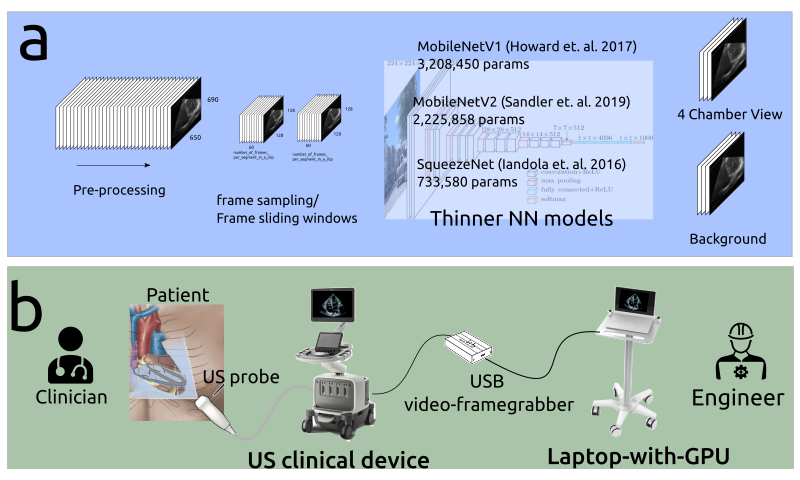
\includegraphics[width=\columnwidth]{../figures/main-figure/versions/drawing-v01}}%%GITHUB
    % {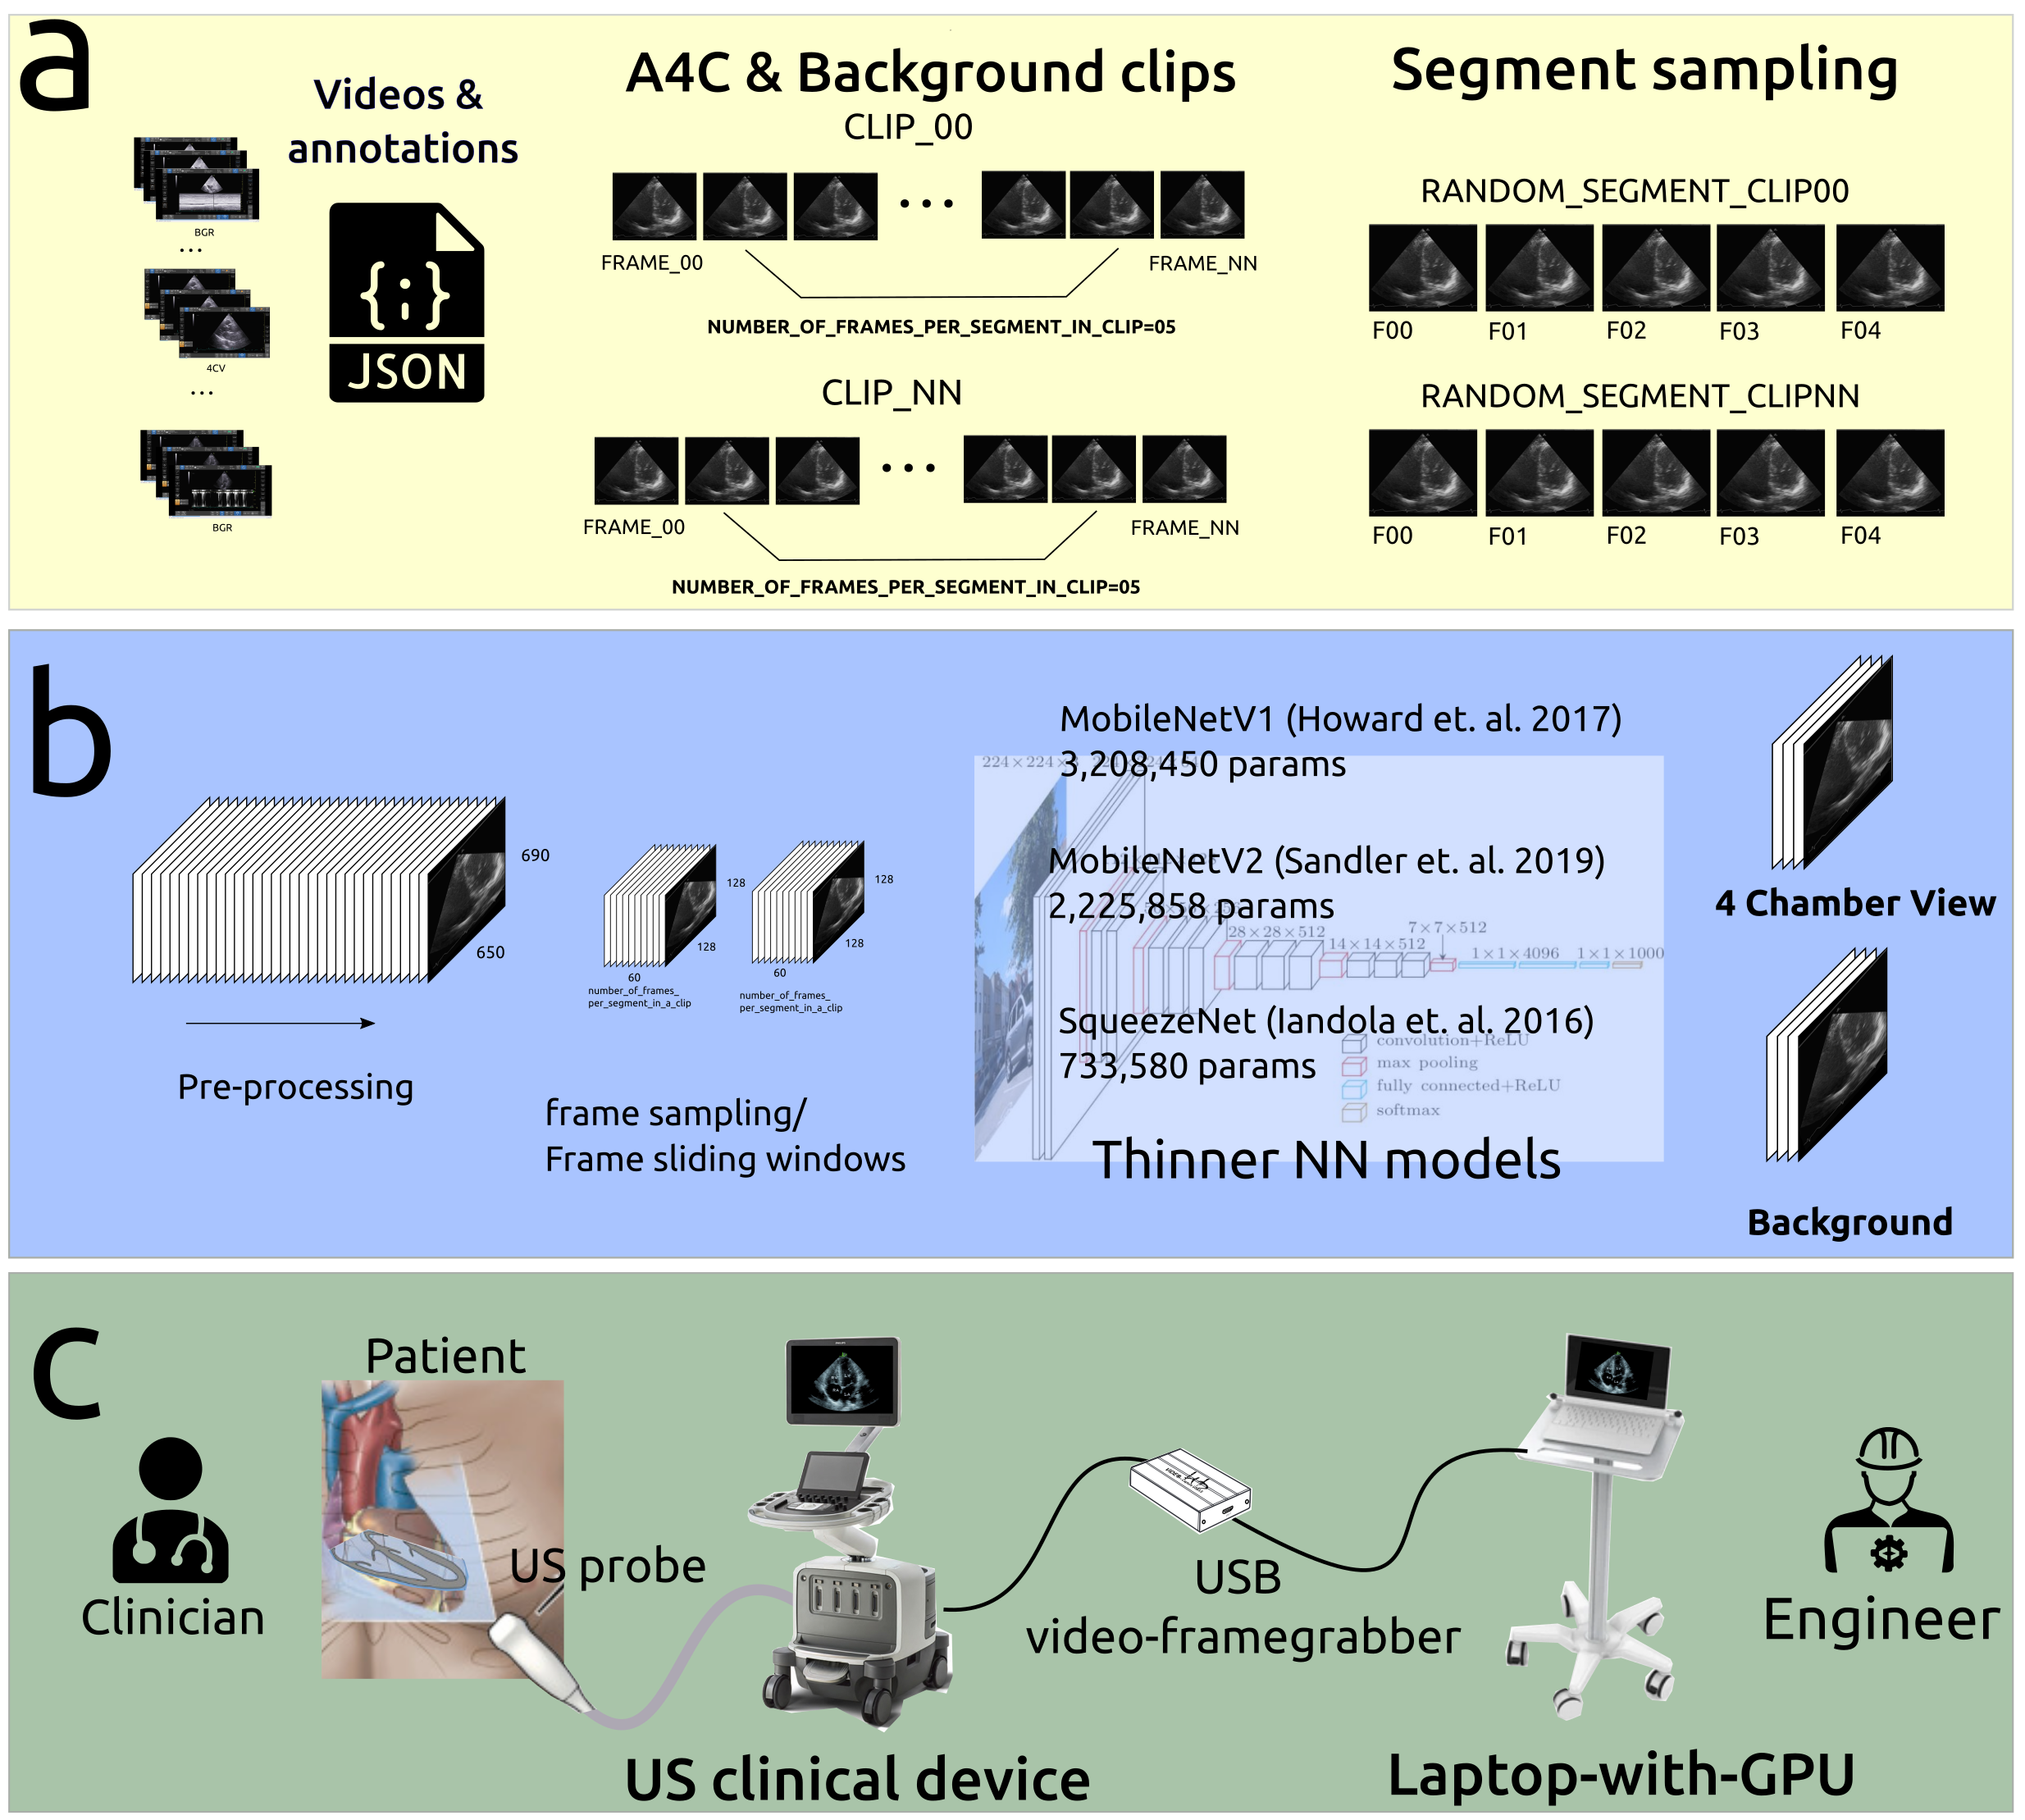
\includegraphics[width=\columnwidth]{figures/main-figure.png}}%%OVERLEAF
    %{\includegraphics[width=\columnwidth]{fig01.png}} %%ARXIV
\end{figure}

\begin{figure}[htbp]
\floatconts
  {fig:heuristics}
  {
      \caption{
          Heuristics for SqueezeNet \citep{iandola2017squeezenet} with dataset of 5 subjects:
          (a) varing batch size and constant number of frames per segment equal to 1, and
          (b) varing number of frames per clip and constant batch size of clips equal to 10.
      }
  }
  {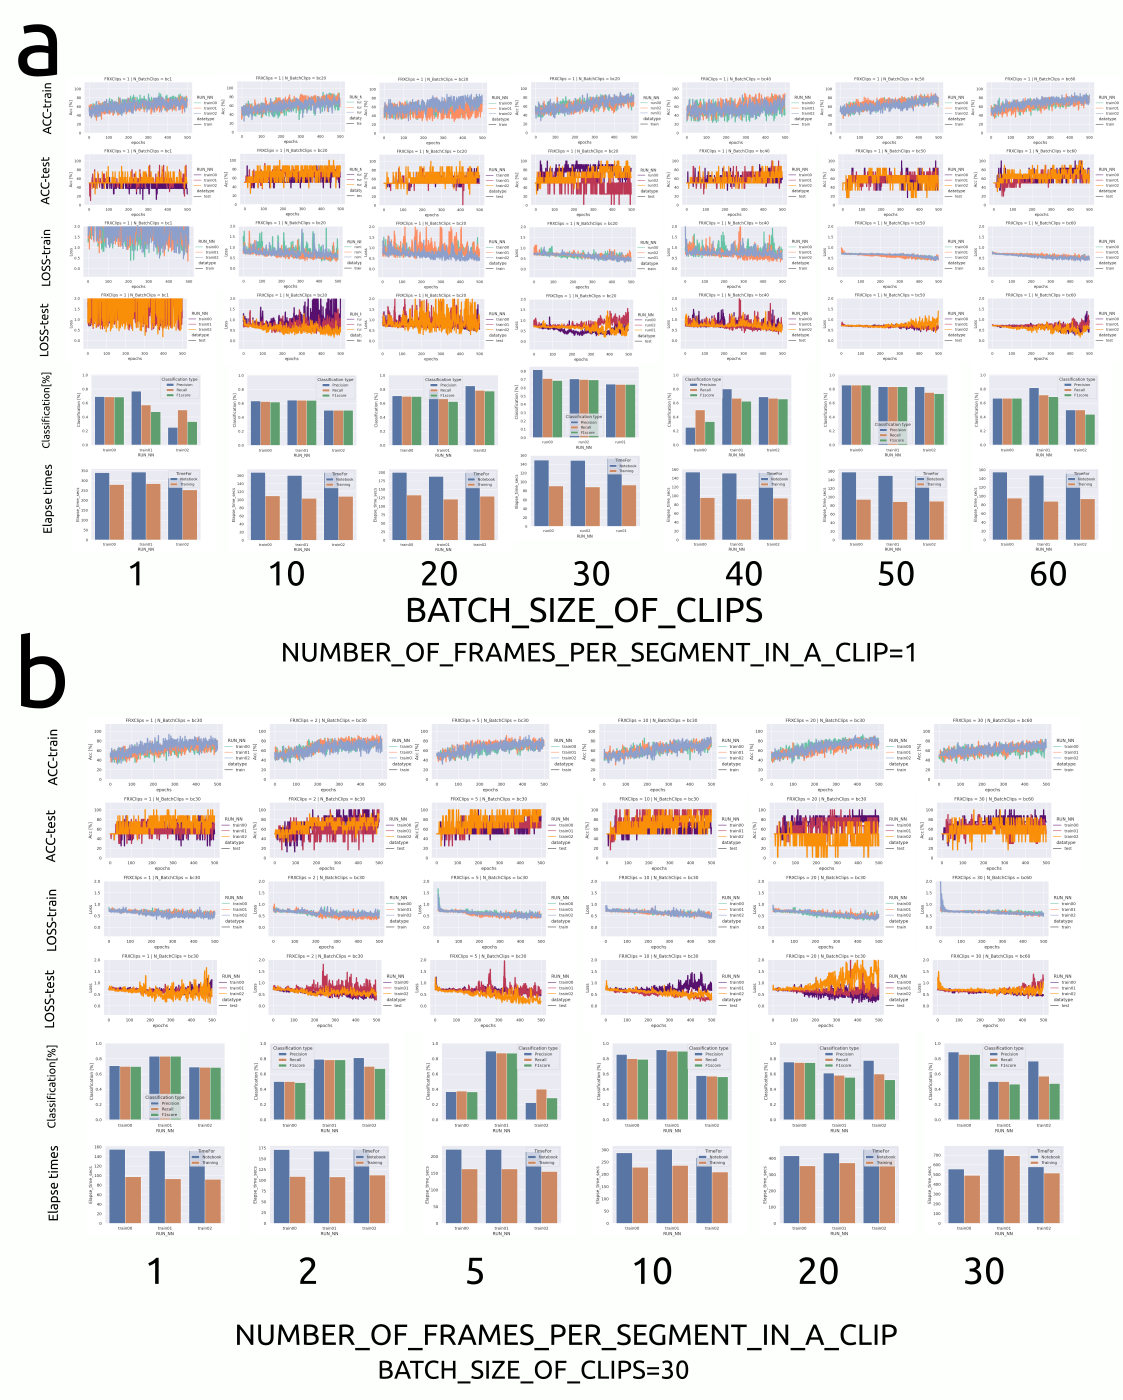
\includegraphics[width=\columnwidth]{../figures/heuristics_results/versions/drawing-v00}}%%GITHUB
    % {\includegraphics[width=\columnwidth]{figures/heuristics.png}}%%OVERLEAF
    %{\includegraphics[width=\columnwidth]{fig01.png}} %%ARXIV
\end{figure}

\section{Conclusions and Future Work}
We presented a machine learning case study, including data selection, validation and management, model selection, validation and low-cost clinical system.
Future work, we will investigate thinner segmentation models, model deployment and clinical validation in the ICU.
%Similarly, we are interested in train models with synthetic Ultrasound images for GE Vivid E9, Hitachi Prosound U7, Philips iE 33 Vision, Siemens SC2000, and Toshiba Artida ultrasound systems \citep{brindise2020unsupervised}.
%2D velocity vector fields of flow blow can help to detect abnormal flow patterns as done in fetal and neonatal echocardiography \citep{Meyers2020}.

%\acks{Acknowledgements go here.}

\bibliography{../references/references}%%%GITHUB
% \bibliography{references}%%%OVERLEAF
%%%%% SELECT ONE OF THE FOLLOWING COMMANDS %%%%%%%%

%%% TEMPLATE FOR PROCEEDINGS TRACK %%%%
%\documentclass[mlmain,twocolumn]{jmlr}

%% TEMPLATE FOR Extended Abstract Track %%%%%%%
\documentclass[mlabstract,twocolumn]{jmlr}
%\documentclass[mlabstract]{jmlr}

%%%%%%%%%%%%%%%%%%%%%%%%%%%%%%%%%%%%%%%%%%%%%%%%%

%%%%%%%%%%%%%%%%%%%%%%%%
% Watermark
%These 4 commands must be removed for the camera-ready version.
\usepackage[hpos=300px,vpos=70px]{draftwatermark}
\SetWatermarkText{\test}
\SetWatermarkScale{1}
\SetWatermarkAngle{0}
%%%%%%%%%%%%%%%%%%%%%%%%%%


%%OVERLEAF
%% Anyone with this link can edit this project
%% https://www.overleaf.com/4969677577xfsfbjqkrnfx


% The following packages will be automatically loaded:
% amsmath, amssymb, natbib, graphicx, url, algorithm2e


%%% WARNING %%%%
%%% 1) Please, use the packages automatically loaded to manage references, write equations, and include figures and algorithms. The use of different packages could create problems in the generation of the camera-ready version. Please, follow the examples provided in this file.
%%% 2) References must be included in a .bib file.
%%% 3) Write your paper in a single .tex file.
%%%

%%%% SOFTWARE %%%%
%%% Many papers have associated code provided. If that is your case, include a link to the code in the paper as usual and provide a link to the code in the following comment too. We will use the link in the next comment when we generate the proceedings.
%%% Link to code: http://?? (only for camera ready)

 %\usepackage{rotating}% for sideways figures and tables
\usepackage{longtable}% for long tables

 % The booktabs package is used by this sample document
 % (it provides \toprule, \midrule and \bottomrule).
 % Remove the next line if you don't require it.
\usepackage{booktabs}
 % The siunitx package is used by this sample document
 % to align numbers in a column by their decimal point.
 % Remove the next line if you don't require it.
\usepackage[load-configurations=version-1]{siunitx} % newer version
 %\usepackage{siunitx}

 % The following command is just for this sample document:
\newcommand{\cs}[1]{\texttt{\char`\\#1}}

 % Define an unnumbered theorem just for this sample document:
\theorembodyfont{\upshape}
\theoremheaderfont{\scshape}
\theorempostheader{:}
\theoremsep{\newline}
\newtheorem*{note}{Note}

%%%% DON'T CHANGE %%%%%%%%%
\jmlrvolume{}
\firstpageno{1}
\editors{List of editors' names}

\jmlryear{2022}
\jmlrworkshop{Machine Learning for Health (ML4H) 2022}

%\editor{Editor's name}
%%%%%%%%%%%%%%%%%%%%%%%%%%%



\title[Short Title]{
%  Full Title of Article\titlebreak This Title Has A Line Break\titletag{\thanks{sample footnote}}
%Real-time AI-empowered echocardiography for Intensive Care Units in low- and middle-income countries %Mon 20 Jun 11:48:09 BST 2022
%Challenges in Real-time AI-empowered echocardiography for Intensive Care Units in low- and middle-income countries. %Fri 19 Aug 15:36:45 BST 2022
Challenges in Real-time AI-empowered echocardiography for Intensive Care Units in low- and middle-income countries: A Machine Learning Case Study %Fri 19 Aug 16:43:05 BST 2022
}

%%%%%%%%%%%%%%%%%%%%%%%%%%%%%%%%%%%%%
% THE MANUSCRIPT, DATA AND CODE MUST BE ANONYMIZED DURING THE REVIEW PROCESS.
% DON'T INCLUDE ANY INFORMATION ABOUT AUTHORS DURING THE REVIEW PROCESS.
% Information about authors (Full names, emails, affiliations) have to be provided only for the submission of the camera-ready version.  Only in that case, you can uncomment and use the next blocks.
%%%%%%%%%%%%%%%%%%%%%%%%%%%%%%%%%%%%%

   \author{
     \Name{Anonymous Author(s)} \Email{email@sample.com}
      \addr Address
   }

 % Use \Name{Author Name} to specify the name.

 % Spaces are used to separate forenames from the surname so that
 % the surnames can be picked up for the page header and copyright footer.

 % If the surname contains spaces, enclose the surname
 % in braces, e.g. \Name{John {Smith Jones}} similarly
 % if the name has a "von" part, e.g \Name{Jane {de Winter}}.
 % If the first letter in the forenames is a diacritic
 % enclose the diacritic in braces, e.g. \Name{{\'E}louise Smith}

 % *** Make sure there's no spurious space before \nametag ***

 % Two authors with the same address
%   \author{\Name{Author Name1\nametag{\thanks{with a note}}} \Email{abc@sample.com}\and
%   \Name{Author Name2} \Email{xyz@sample.com}\\
%   \addr Address}

  %Three or more authors with the same address:
%   \author{\Name{Author Name1} \Email{an1@sample.com}\\
%   \Name{Author Name2} \Email{an2@sample.com}\\
%   \Name{Author Name3} \Email{an3@sample.com}\\
%   \Name{Author Name4} \Email{an4@sample.com}\\
%   \Name{Author Name5} \Email{an5@sample.com}\\
%   \Name{Author Name6} \Email{an6@sample.com}\\
%   \Name{Author Name7} \Email{an7@sample.com}\\
%   \Name{Author Name8} \Email{an8@sample.com}\\
%   \Name{Author Name9} \Email{an9@sample.com}\\
%   \Name{Author Name10} \Email{an10@sample.com}\\
%   \Name{Author Name11} \Email{an11@sample.com}\\
%   \Name{Author Name12} \Email{an12@sample.com}\\
%   \Name{Author Name13} \Email{an13@sample.com}\\
%   \Name{Author Name14} \Email{an14@sample.com}\\
%   \addr Address}


%%  Authors with different addresses:
%  \author{\Name{Author Name1} \Email{abc@sample.com}\\
%  \addr Address 1
%  \AND
%  \Name{Author Name2} \Email{xyz@sample.com}\\
%  \addr Address 2
% }



\begin{document}

\maketitle

\begin{abstract}
We present a machine learning case study on the current and future challenges of implementing a real-time AI-empowered echocardiography system for ICU in LMICs.
We present reproducible heuristics from a small video dataset of 31 subjects in the ICU, data preparation, curation and labelling, model selection, validation and deployment.
The code and other resources to reproduce this work are available at \url{https://github.com/vital-ultrasound/echocardiography}.
\end{abstract}
\begin{keywords}
deep learning; echocardiography; real-time artificial intelligence;
\end{keywords}

\section{Introduction}
\label{sec:intro}
Echocardiography is an important clinical procedure in Intensive Care Units (ICU) because of the advances of Ultrasound (US) such as portability, low cost, low radiation and its real-time capabilities to access cardiac anatomy \citep{Feigenbaum1996, Vieillard-Baron2008, singh2007, cambell2018}.
Despite that, there various challenges in the current clinical procedures in the ICU:
\begin{itemize}
\setlength\itemsep{0em}
\item Intra-view variability of echocardiograms (physiological variations of subjects and acquisition parameters) and inter-observer variability of expertise for sonographer and radiologist \citep{khamis2017, Feigenbaum1996, field2011},
\item Inter-view similarity of echocardiograms (similar views of valve motion, wall motion, left ventricle, etc) and transducer position during acquisition \citep{zhang2018},
\item Redundant information in the clinical echo system (icons, date, frame rate, etc) \citep{khamis2017} and variation of Ultrasound images from different clinical US systems \citep{brindise2020unsupervised}, and
\item Limited number of expert clinicians to perform US imaging analysis and to provide accurate diagnosis, as well as equipment and hospitalisation requirements in low- and middle-income countries (LMICs) \citep{hao2021-wellcome, 2021-huyNhat-vanHao-in-FAIR-MICCAI}.
\end{itemize}
One promising approach to address such challenges is with the application of Artificial Intelligence to echocardiography.
AI-empowered echocardiography has been successful for detection of different apical views, inter-observer variability of sonographer's expertise, implementation of one-stop AI models with multimodal imaging (US, MRI and clinical data), detection of high risk or low risk of heart failure or automatic detection of endocardial border detection and left ventricle assessment in 2D echocardiography videos \citep{tromp2022, zhang2022-mdpi, behnami2020, ono2022}.
However, there is little to none studies on how real-time AI-empowered echocardiography might impact the ICU in LMICs.
Particularly, how good machine learning practices (data curation, code implementation, model selection, training and tuning; model validation and inference) are addressing challenges on real-time AI-empowered echocardiography in the ICU in LMICs.

This work presents (a) a scoping review of AI-empowered echocardiography for ICU in LMICs and (b) real-time AI-empowered echocardiography, (c) a machine learning case of study of US image classification using deep learning of four chamber views from curated data from LMICs and (d) conclusions future work.
%appendix with further material.

% \subsection{AI-empowered echocardiography}
% Tromp et al. classified a dataset of 1145 2D echocardiography videos as apical 4 chamber (A4C) view, apical 2 chamber (A2C) view, parasternal long axis (PLAX) view, or 2D other views and focused versions of the main views \citep{tromp2022}.
% Authors used CNN of four layers, dense network and softmax output layer, trained with categorical cross-entropy loss function, then a second classifier of an unsupervised deep learning clustering CNN, trained with mean square error and Kullback-Leibler loss functions \citep{tromp2022}.
% %For the remaining dataset (2,126 PSAX-PM echo cines), while the LV segmentation is not available, the ground truth LVEF values are acquired from the patients’ archived information.

% \citet{zhang2022-mdpi}
% reviewed AI's applications in left ventricular systolic function (LVEF) and global longitudinal strain (GLS), pointing out its dependency to the sonographers's expertise (inter-observer variability) and post-processing and variability in different US devices.
% \citet{zhang2022-mdpi} pointed the challenges of AI-enhanced echocargiografy for interpretability of results and its sensitivity to sample shortage, to which authors mention about the potentials of multimodal imaging (us, mri and clinical data) to improve detection rate of diseases.

% \citet{behnami2020} applied DenseNet-like network for feature learning and RNN unit with bidirectional Gated Recurrent Units to alleviate loss of information from the earlier frames of echos to automatically detect high risk or low risk of heart failure with reduced ejection fraction with an overall accuracy of 83.15\%, precision of 82.6\% and recall of 81.1\%.
% \citet{behnami2020} mentioned that EF is highly user-dependant to which they propose to collect more data,

% \citet{liu2021JMIA} proposed pyramid local attention neural network (PLANet) to improve segmentation performance of automatic methods in 2D echocardiography.
% PLANet was evaluated with CAMUS and sub-EchoNet-Dynamic datasets, showing a better performance against geometric and clinical metrics.

% \citet{ulloaCerna2021} made use of DNN to learn spatiotemporal features from echocardiography video data to enhance clinical prediction of 1 yr all-cause mortality where video echo data linked to EHR data that included hand-crafted echocardiography-derived measurements (EDMs), additional clinical variables and individual outcomes.
% The DNN model presents "superior prediction performance" over four cardiologist and two benchmark clinical models: the pooled cohort equations (PCE) and Seattle Heart Failure (SHF) risk score \citep{ulloaCerna2021}.
% \citet{ulloaCerna2021} used "full, raw (annotation-free) echocardiographic videos to make predictions by learning from more than 812,278 clinically acquired echocardiography videos of the heart (50 million images)."

% \citet{jafari2021} pointed out the challenges of obtained high quality for less experience operators and the hight variability or echo quality adn cardiovascular structures across different patients to which authors proposed "Bayesian deep learning approach for fully automatic LVEF estimation based on segmentation of the left ventricle (LV) in parasternal short-axis papillary muscles (PSAX-PM) level".
% \citet{jafari2021} made use of 2,680 patients with PSAX-PM echo cine acquired by a variety of ultrasound devices, namely iE33, Vivid i/7/9/95, Sonosite, and Sequoia (only 554 echo cines were considered as ground truth with LV mask delineated by an experienced level III echocardiographer).

% Ono et al. applied different models where Unet++ demonstrated good performance for automatic endocardial border detection and left ventrical assessment in 2D echocardiography videos \citep{ono2022}.
% The datasets to train networks was made of 2798 images from 118 videos of which 22 videos with 465 frames were for 4CV \citep{ono2022}.
% Ono et al. also touched on the challenges of providing explainable AI for US imaging.


\section{AI-empowered echocardiography for ICU in LMICs}
\citet{hanson2001} reviewed various applications of AI in the ICU where real-time analysis of waveforms of electrocardiograms and electroencephalograms using neural network were used to identify cardiac ischemia and diagnosis myocardial ischemia.
\citet{hanson2001} also reviewed various ICU scenarios where variables such as central venous pressure (CVP), left ventricular ejection fraction (EF), heart rate (HR), hemoglobin (HGB) and oxygen saturation (O2sat) were used with Bayesian networks to provide probabilistic cardiac output.
%\citet{hanson2001} also touched on data visualisation to demonstrate the hypothetical ICU for large number of patients (head injury, sepsis, acute respiratory distress syndrome, etc).
\citet{Ghorbani-DigitalMedicineNature-JAN2020} reported how deep learning models predicts systematic phenotypes which are difficult for human interpreters from echocardiogram images, the extraction of labels local structures and features (e.g. pacemaker lead, dilation of left atrium, hypertrophy for left ventricular) and labels from the physician-interpreted report (e.g, catheters, pacemaker, and defibrillator leads).
%to predict age, sex, weight and height
%and make use of such models
%Authors trained CCN models with 2.6 million echocardiogram images from 2850 patients with
\citet{CHEEMA2021JACCCaseReports} presented five cases covid-19 intensive care unit (ICU) to illustrate "how decision making affect in patient care" and how the use of AI-enabled provided real-time guidance to acquire desired cardiac US with the steering of user's transducer position and hand movement.
Recently, \citet{hong2022} reviewed 673 papers that made use of machine learning to help for clinical decision in the ICU, of these studies the majority used supervised learning (91\%) and few of them applied unsupervised learning and reinforcement learning.
Similarly, \citet{hong2022} identified 20 of the most frequent variables in the ICU, being the top five (age, sex, heart rate, respiratory rate, and pH) in machine learning pipelines.
\citet{hong2022} mentioned that typical outcomes in the ICU are mortality, survival, and long-term quality of life and included typical patient outcomes, specific diseases, and stay of time evaluation and specific diseases where the most studied are sepsis, infection and kidney injury.
%For specific diseases, the most studied are sepsis, infection and kidney injury; and trends with liver diseases and severe cancerl and others like cardica diseases, brain diseases;
However, there is few research on AI-empowered echocardiography for ICU in LMICs where, for instance, \cite{2021-huyNhat-vanHao-in-FAIR-MICCAI} reported challenges in resourced limited ICUs including: infrastructure, education and personnel, data pipelines, regulation and trust in AI.
Also, \cite{2021-kerdegari-Applied-Sciences-MDPI, 2021-kerdegari-ISBI-IEEE, 2021-huyNhat-kerdegari-in-FAIR-MICCAI} presented a deep-learning lung US pathology classifier for ICU patient in LMIC, stating the challenges of data imbalance, integration of technology and IT infrastructure of the ICU in LMIC.

\section{Real-time AI-empowwered echocardiography}
%In terms of real-time analysis of echocardigraphy, , 
\citet{woudenberg2018} trained an DenseNet-LSTM with 2K clips of 4 chamber view in which the real-time system made use of 10 input frames and reported a latency of 352.91ms.
\citet{toussaint2018-MICCAI} proposed ResNet18-SP trained with 85k frames of Fetal US imaging, reporting real-time performance at inference time of 40 m$s$ per image or $\sim$20Hz.
\citet{ostvik2021-TMI} proposed Echo-PWC-Net trained with Synthetic/Simulated/Clinical, reporting real-time performance with 7 frames for the input.
Recently, \citet{wu2022} applied baselines of UNET with temporal context-aware encoder (TCE) and bidirectional spatiotemporal semantics fusion (BSSF) modules to EchoDynamic datasets (10030 video sequences with of 200 frames of 112x112 pixes) and CAMUS datasets  (450 video with 20 frames of 778x594 pixels), reporting metrics of Dice score (DS), Hausdorff Distance (HD), and area under the curve (AUC).
Similarly, \citet{wu2022} presented speed analysis to ensure low latency and real-time performance for eight methods using calculations number FLOPS (G), number of parameters (M) and speed ($ms/f$).
%which lowest one was 32 $ms/f$.

\subsection{Classification of echochardiograms}
\citet{khamis2017} considered 309 clinical echocardiogram of apical views which were visually classified and labelled by two experts into three classes: 103 a2c views, 103 a4c views and 103 alx views to then applied spatio-temporal feature extraction (Cuboic Detector) and supervised learning dictionary (LC-KSVD) resulting in an overall recognition rate of 95\%.
\citet{woudenberg2018} applied DenseNet and LSTM to extract temporal information on sequences of 16K echo cine frames to classify 14 heart views with an average accuracy of 92.35\%.
%\citet{woudenberg2018} implemented a Tensorflow runner that performs contrast enhancement to then sent each frame to three identical CNNs running in separated threads to prevent lag during inference times.
%Then a shared buffer collects extracted features from CNNs to then awake the thread for the LSTM network from the previous ten frames to produce classification and quality prediction.
\citet{woudenberg2018} also presents timing diagrams to quantify frame arrival and real-time performance to operate at 30 frames per second, while providing feedback with a mean latency of 352.91 ± 38.27 m$s$ when measured from the middle of the ten-frame sequence.
\citet{zhang2018} performed view classification with 277 echocardiograms to create a 23-class models (including a4c no occlusions, a4c occluded LA, a4c occluded LV, etc) using 13-layer CNN with 5-fold cross-validation for accuracy assessment and resulting in 84\% for overall accuracy where challenges for partial obscured LVs for a2c, a3c and a4c.
Similarly, \citet{zhang2018} applied U-net to segment 5 views (a2c, a3c, a4c, PSAX, PLAX) and CNN model for 3 cardiac diseases with the use of A4c capturing most of the information for the diseases.

\subsection{Thinner neural networks to classify US images} \label{subsec:thinnerNets}
\citet{baumgartner2017-IEEETransMedImag} proposed SonoNet which is a VGG-based architecture, having the same first 13 layers of VGG16, and SmallNet, loosely inspired by AlexNet, for real-time detection and bounding box localisation of standard views in freehand fetal US.
\citet{toussaint2018-MICCAI} applied four feature extraction networks couple with batchnormalization and soft proposal layer (VGG13-SP, VGG16-SP, ResNet18-SP, ResNet34-SP), resulting in 0.912 of average accuracy over six classes of fetal US views with ResNet18-SP.
\citet{Al-Dhabyani2019-IJACSA} applied AlexNet and transfer learning of four architectures (VGG16, Inception, ResNet, and NASNet) without augmentation and with three augmentation techniques to perform tumor classification of breast ultrasound imaging.
Authors stated that transfer learning with NASNet presented the best accuracy with 99\% using BUSI+B datasets with DAGAN augmentation.
\citet{xie2020-physics-in-medicine-biology} proposed a dual-sampling convolutional neural network (DSCNN) for US image breast cancer classification, being DSCNN more efficient than AlexNet, VGG16, ResNet18, GoogleNet and EfficientNet.
Recently, \citet{snider2022-ScientificReports} reported summaries of CNN heuristics to detect shrapnel in US images, including layer activators, 2D CNN layer architectures, model optimisers dense nodes, and the effect of image augmentation and dropout rate and epoch number.
Similarly, \citet{boice2022-in-jimaging} proposed ShrapML, a CNN model to detect shrapnel in US imaging.
Authors compared ShrapML (8layers--6CNN,2FC, 0.43 million of parameters) against DarkNet19, GoogleNet, MobileNetv2 and SqueezeNet, being ShrapML 10x faster than MobileNet2 which offered the highest accuracy.

\section{Machine learning case study}

\subsection{Dataset}
Echocardiography videos of 31 subjects in the ICU were considered for this work which were collected by four radiologists using the clinical devices: GE Venue Go machine and GE convex probe C1-5-D.
The 31 subjects has the following demographics:
Sex: \% (Male): 58.1\%;
Age: mean, years (std): 38.70 (16.08);
Weight: mean, Kg (std): 61.51 (15.06);
Height: mean, m (std): 1.62 (0.07);
BMI: mean (std): 23.80 (4.30);
Sepsis \% (with): 61.3\%;
Dengue \% (with): 54.8\%, and
Tetanus \% (with): 87.1\%.
See \appendixref{apd:datasets} for further details on the demographics of the dataset, including the complete dataset of 87 subjects.

\subsubsection{Ethics statement}
This study was approved by the Oxford Tropical Research Ethics Committee (OxTREC) and the HTD Institutional Review Boards (Hospital of Tropical Diseases).
All participants gave written informed consent to participate before enrollment.

\subsubsection{Data annotation, validation and management}
Timestamps of 4 chamber views of video files from 31 subjects were annotated by one research clinician of 10 years of experience using VGG Image Annotator (VIA).
Then the same clinician  and one researcher validated annotations in a round of two iterations where few filenames timestamps were fixed.

\subsection{Model selection and heuristics}
Considering \sectionref{subsec:thinnerNets}, we selected four thinner Neural Networks for our ML study: MobileNetV1 \citep{2017-howared_CoRR_MobileNetV1} 3,208,450; MobileNetV2 \citep{Sandler_2018_CVPR_MobileNetV2} 2,225,858; SqueezeNet \citep{iandola2017squeezenet} 733,580 and ShrapML \citep{boice2022-in-jimaging} 430,000 (networks and parameters, respectively).
We then performed heuristics for each model to understand their performance for different hyperparameters (datasize, augmentations and clip length) as shown in \figureref{fig:heuristics}.
See \appendixref{apd:heuristics} for further details on each model.
%See \figureref{fig:SqueezeNetTrainingResults} for further results on SqueezeNet Training performance.
%\begin{table}[htbp]
%\floatconts
%  {tab:example}%
%  {\caption{Thinner Neural Networks}}%
%{\begin{tabular}{lllll}
%\textbf{Networks} & Parameters \\
%MobileNetV1 \citep{2017-howared_CoRR_MobileNetV1} & 3,208,450    \\
%MobileNetV2 \citep{Sandler_2018_CVPR_MobileNetV2} & 2,225,858   \\
%SqueezeNet \citep{iandola2017squeezenet} & 733,580 \\
%ShrapML \citep{boice2022-in-jimaging} & 430,000
%\end{tabular}}
%\end{table}
\begin{figure}[htbp]
\floatconts
  {fig:main-figure}
  {\caption{
      Proposed low-cost clinical system for real-time AI-empowered echocardiography:
      (a) deep-learning pipeline with thinner NNs, and
      (b) clinical system: Epiq Q7, cardiac probe X5-1, USB video-frame grabber and 16GB GeForce RTX 3080 GPU Laptop
    }
  }
  {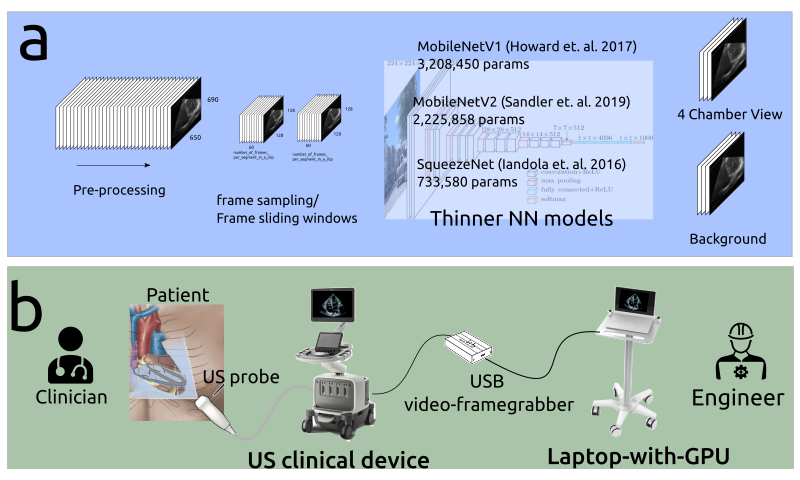
\includegraphics[width=\columnwidth]{../figures/main-figure/versions/drawing-v01}}%%GITHUB
    % {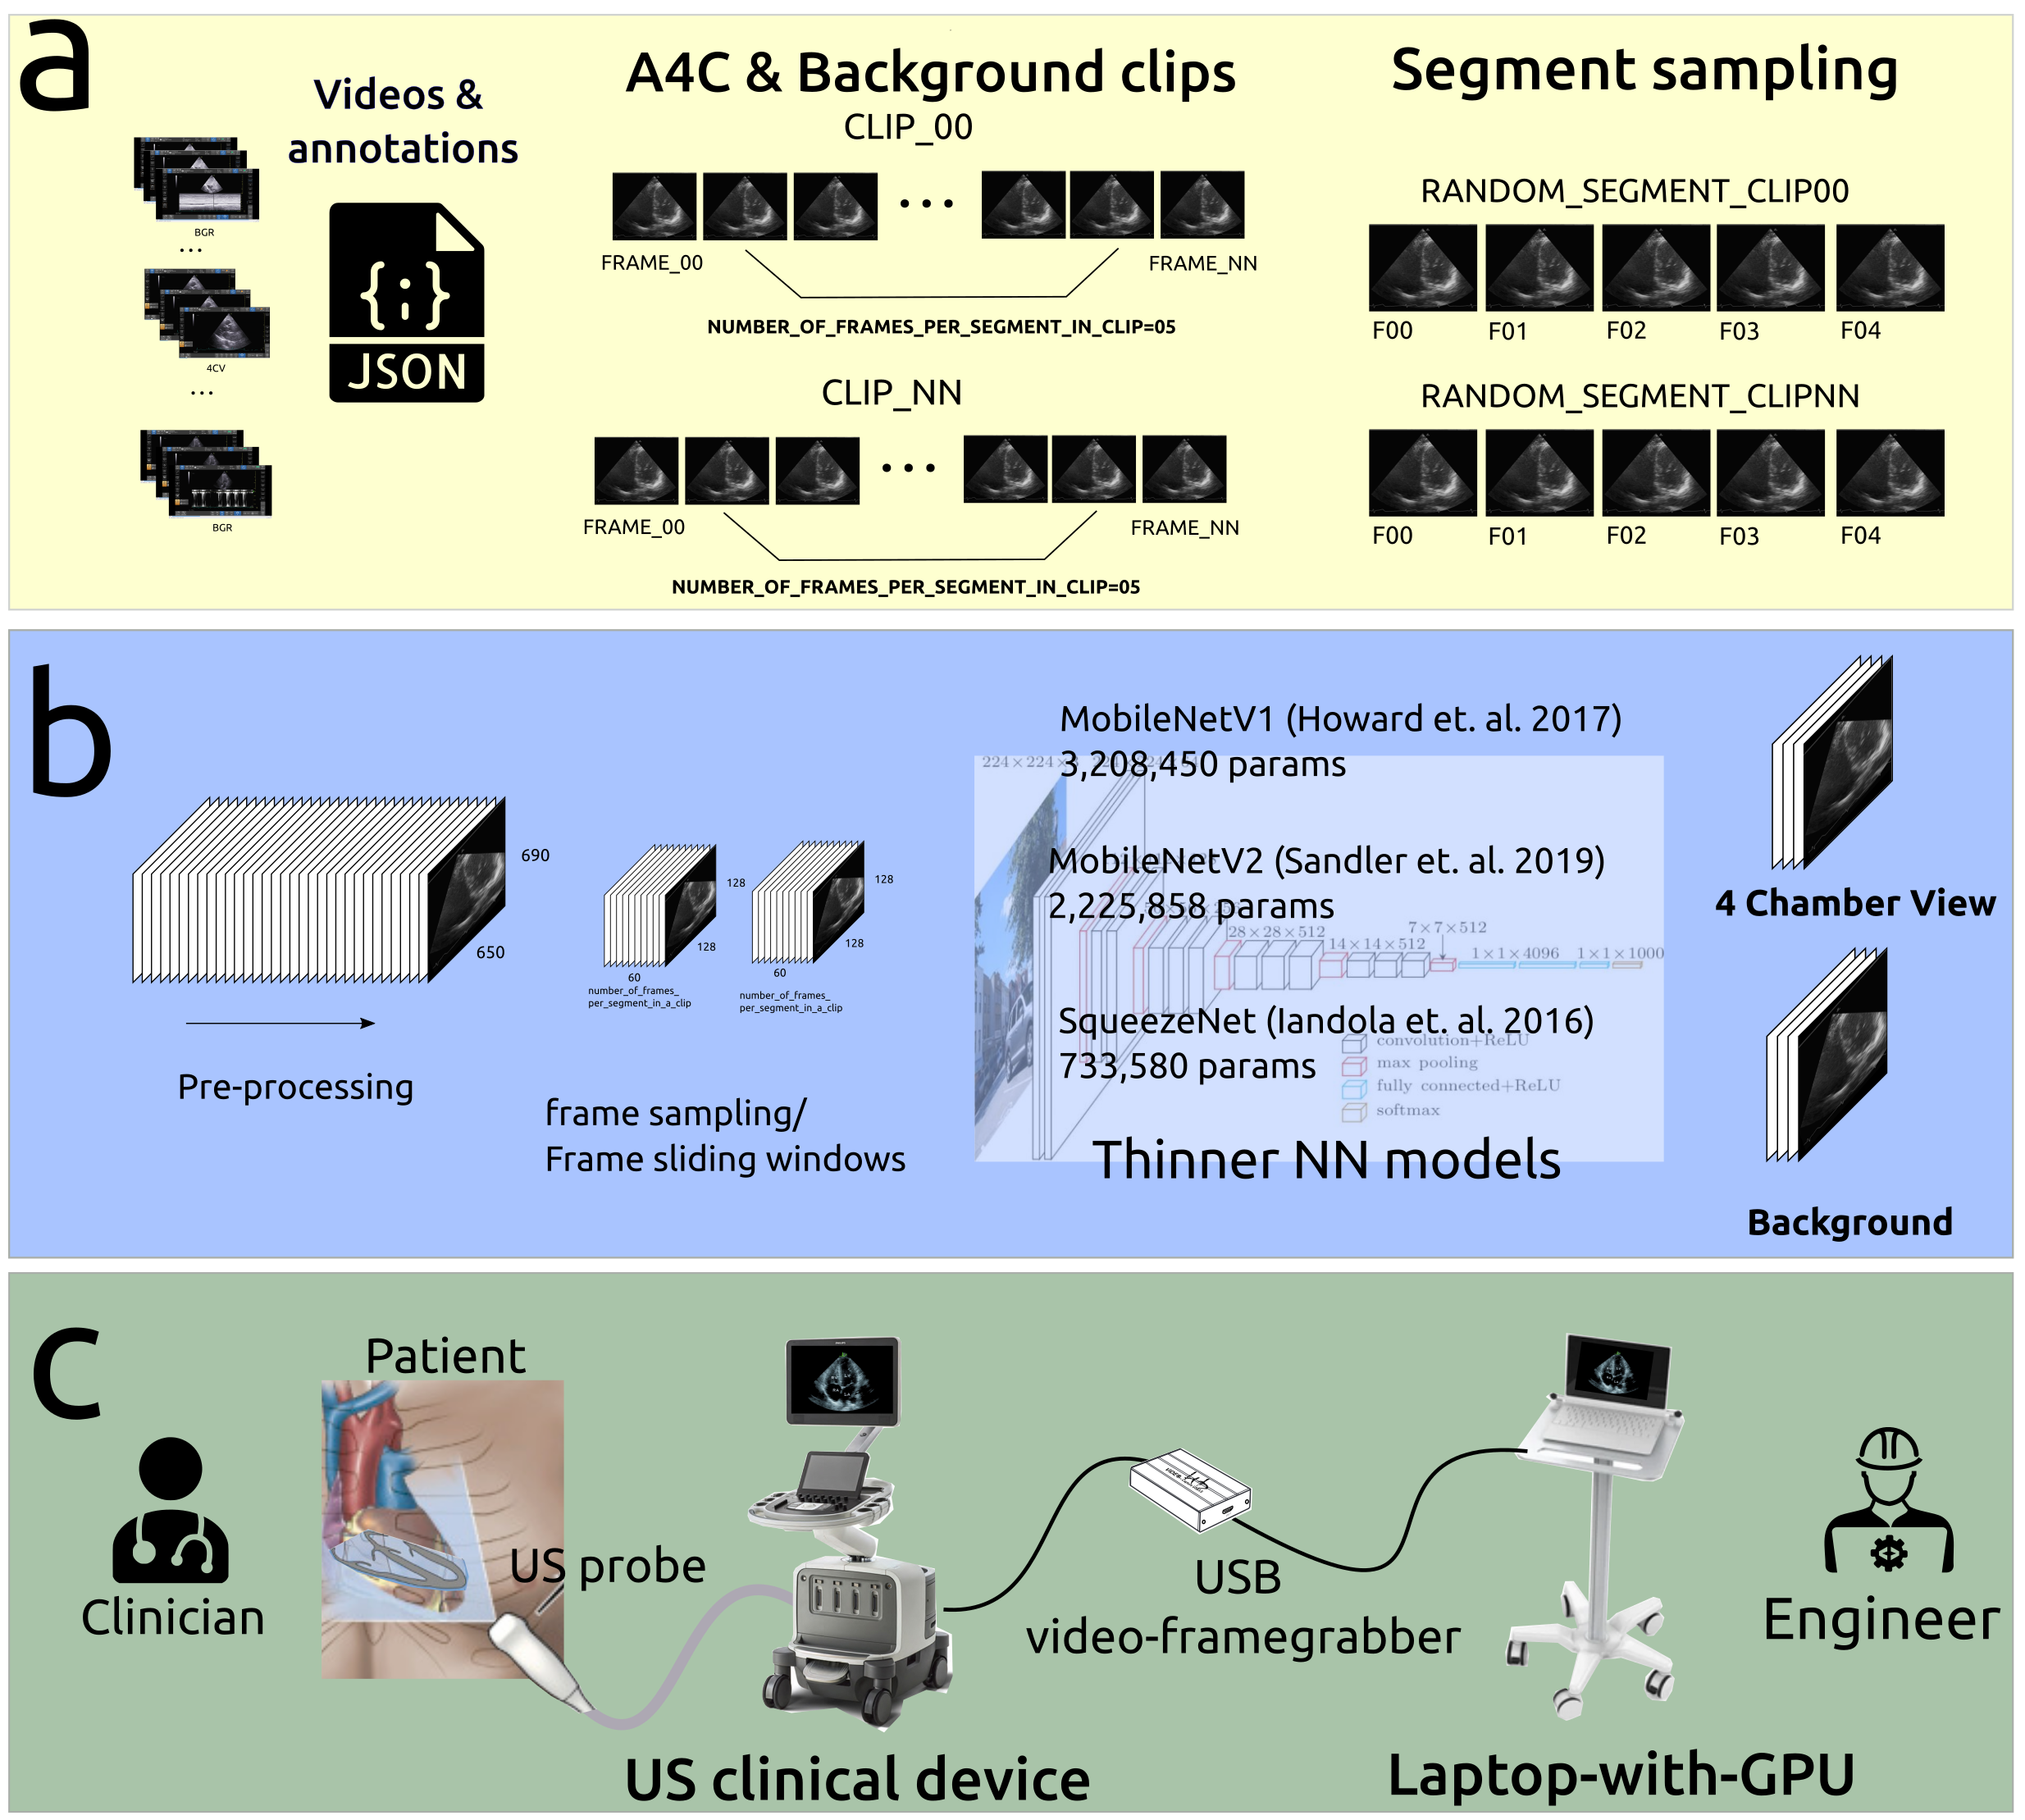
\includegraphics[width=\columnwidth]{figures/main-figure.png}}%%OVERLEAF
    %{\includegraphics[width=\columnwidth]{fig01.png}} %%ARXIV
\end{figure}

\begin{figure}[htbp]
\floatconts
  {fig:heuristics}
  {
      \caption{
          Heuristics for SqueezeNet \citep{iandola2017squeezenet} with dataset of 5 subjects:
          (a) varing batch size and constant number of frames per segment equal to 1, and
          (b) varing number of frames per clip and constant batch size of clips equal to 10.
      }
  }
  {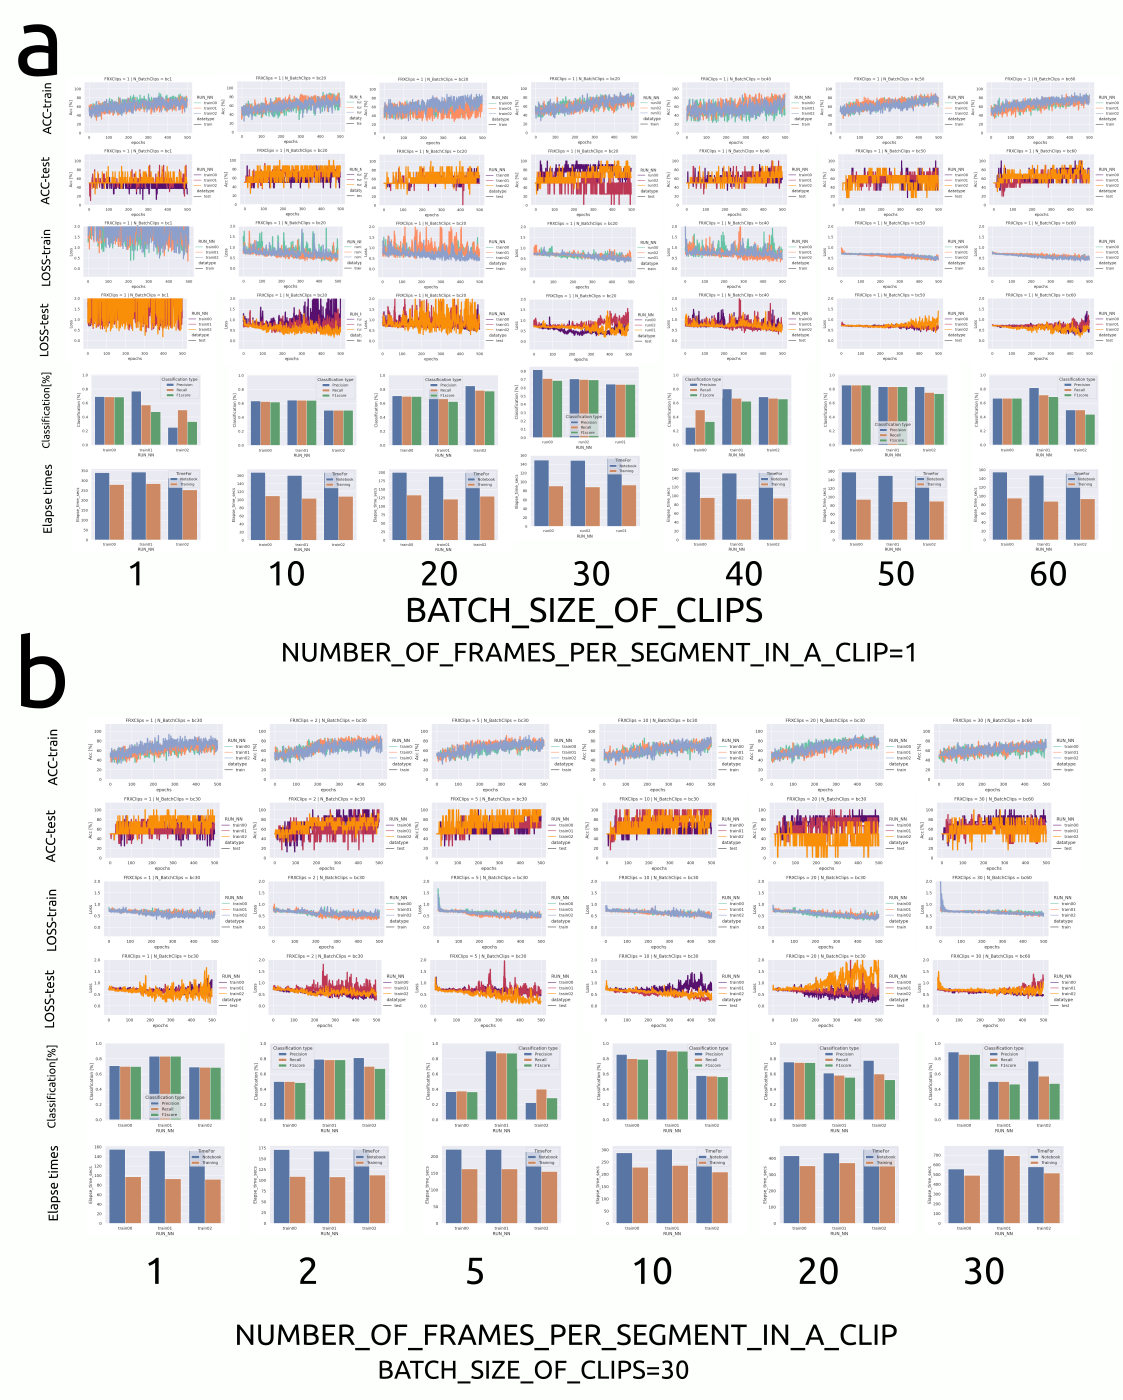
\includegraphics[width=\columnwidth]{../figures/heuristics_results/versions/drawing-v00}}%%GITHUB
    % {\includegraphics[width=\columnwidth]{figures/heuristics.png}}%%OVERLEAF
    %{\includegraphics[width=\columnwidth]{fig01.png}} %%ARXIV
\end{figure}

\section{Conclusions and Future Work}
We presented a machine learning case study, including data selection, validation and management, model selection, validation and low-cost clinical system.
Future work, we will investigate thinner segmentation models, model deployment and clinical validation in the ICU.
%Similarly, we are interested in train models with synthetic Ultrasound images for GE Vivid E9, Hitachi Prosound U7, Philips iE 33 Vision, Siemens SC2000, and Toshiba Artida ultrasound systems \citep{brindise2020unsupervised}.
%2D velocity vector fields of flow blow can help to detect abnormal flow patterns as done in fetal and neonatal echocardiography \citep{Meyers2020}.

%\acks{Acknowledgements go here.}

\bibliography{../references/references}%%%GITHUB
% \bibliography{references}%%%OVERLEAF
%\input{main.bbl}%%%ARXIV

\appendix

\section{Datasets}\label{apd:datasets}
\figureref{fig:demographics} illustrates demographics for sex, age, BMI, sepsis and denque for the complete dataset and the 31 subjects considered for this work.
\begin{figure}[htbp]
\floatconts
  {fig:demographics}
  {\caption{Patient demographics.}} %Figure is adapted from the works of %\cite{}.
  {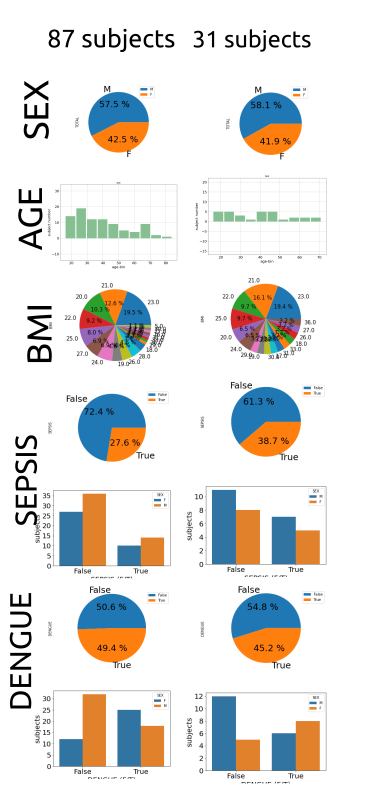
\includegraphics[width=\columnwidth]{../figures/patient-demographics-and-diseases/versions/drawing-v01}}%%GITHUB
    % {\includegraphics[width=\columnwidth]{figures/patient-demographics-and-diseases.png}}%%OVERLEAF
    %{\includegraphics[width=\columnwidth]{fig01.png}} %%ARXIV
\end{figure}

\section{Heuristics of model selection} \label{apd:heuristics}
\figureref{fig:ThinnerNeuralNetsResults} illustratres heristics for accuraty, train, classification and elapse times of 5 and 31 subjects.
\begin{figure*}[ht]
\floatconts
  {fig:ThinnerNeuralNetsResults}
%  {\caption{Heuristics for 5 and 33 subjects with 10 frames per clip and 25 batch size of clips using SqueezeNet \citep{iandola2017squeezenet}.}}
  {\caption{
    Heuristics for 5 and 31 subjects with 1 frames per clip and 20 batch size of clips for
    MobileNetV1 \citep{2017-howared_CoRR_MobileNetV1}, MobileNetV2 \citep{Sandler_2018_CVPR_MobileNetV2}, and SqueezeNet \citep{iandola2017squeezenet} 733,580
    %and ShrapML \citep{boice2022-in-jimaging} 430,000
          }.
  }
  {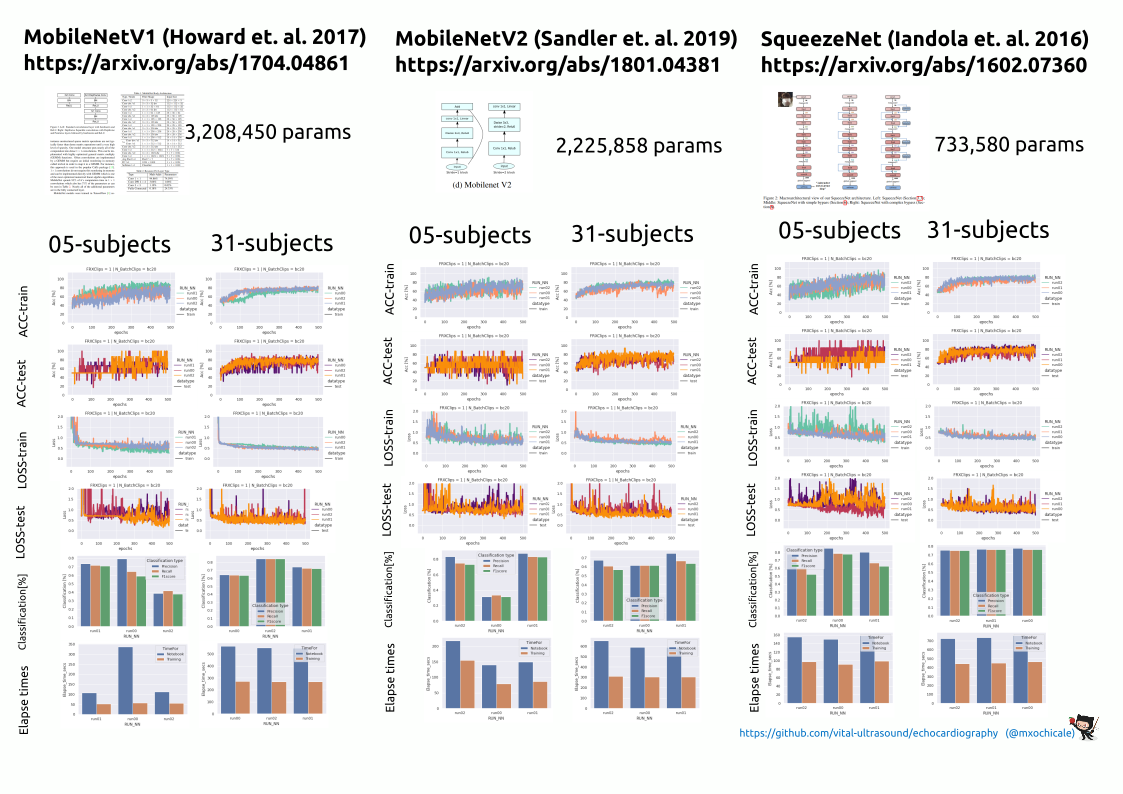
\includegraphics[width=\textwidth]{../figures/comparing-NETS-for-USviewclassification/versions/drawing-v00}}%%GITHUB
    % {\includegraphics[width=\columnwidth]{figures/squeezenet-05-33-subjects.png}}%%OVERLEAF
    %{\includegraphics[width=\columnwidth]{fig01.png}} %%ARXIV
\end{figure*}

\end{document}

%%%ARXIV

\appendix

\section{Datasets}\label{apd:datasets}
\figureref{fig:demographics} illustrates demographics for sex, age, BMI, sepsis and denque for the complete dataset and the 31 subjects considered for this work.
\begin{figure}[htbp]
\floatconts
  {fig:demographics}
  {\caption{Patient demographics.}} %Figure is adapted from the works of %\cite{}.
  {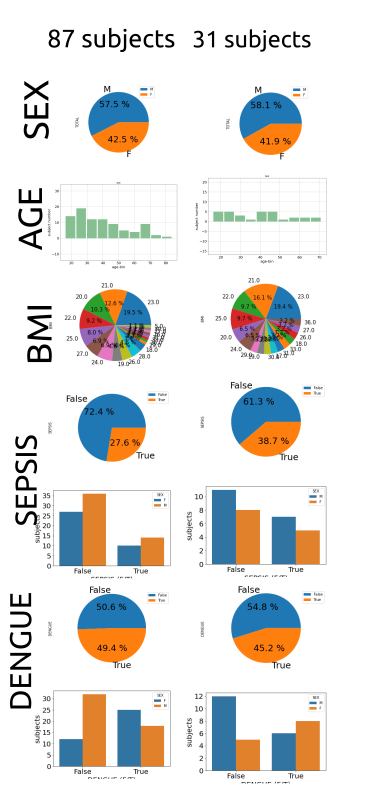
\includegraphics[width=\columnwidth]{../figures/patient-demographics-and-diseases/versions/drawing-v01}}%%GITHUB
    % {\includegraphics[width=\columnwidth]{figures/patient-demographics-and-diseases.png}}%%OVERLEAF
    %{\includegraphics[width=\columnwidth]{fig01.png}} %%ARXIV
\end{figure}

\section{Heuristics of model selection} \label{apd:heuristics}
\figureref{fig:ThinnerNeuralNetsResults} illustratres heristics for accuraty, train, classification and elapse times of 5 and 31 subjects.
\begin{figure*}[ht]
\floatconts
  {fig:ThinnerNeuralNetsResults}
%  {\caption{Heuristics for 5 and 33 subjects with 10 frames per clip and 25 batch size of clips using SqueezeNet \citep{iandola2017squeezenet}.}}
  {\caption{
    Heuristics for 5 and 31 subjects with 1 frames per clip and 20 batch size of clips for
    MobileNetV1 \citep{2017-howared_CoRR_MobileNetV1}, MobileNetV2 \citep{Sandler_2018_CVPR_MobileNetV2}, and SqueezeNet \citep{iandola2017squeezenet} 733,580
    %and ShrapML \citep{boice2022-in-jimaging} 430,000
          }.
  }
  {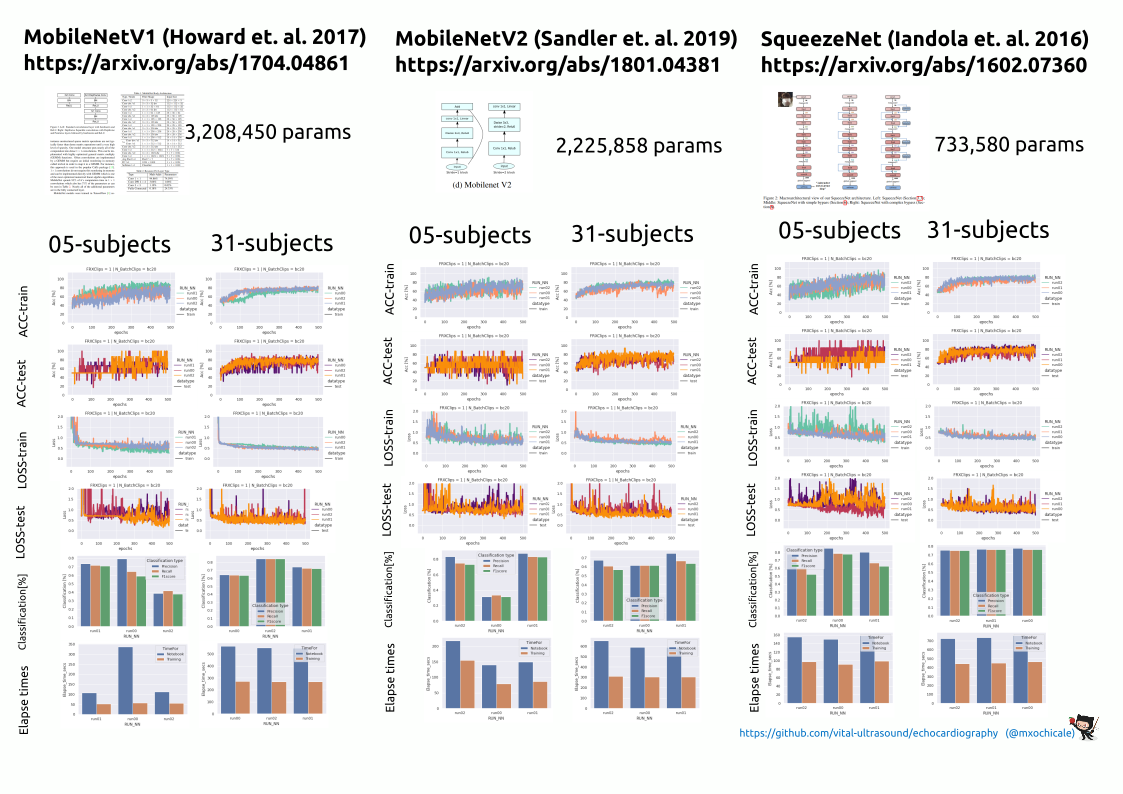
\includegraphics[width=\textwidth]{../figures/comparing-NETS-for-USviewclassification/versions/drawing-v00}}%%GITHUB
    % {\includegraphics[width=\columnwidth]{figures/squeezenet-05-33-subjects.png}}%%OVERLEAF
    %{\includegraphics[width=\columnwidth]{fig01.png}} %%ARXIV
\end{figure*}

\end{document}

%%%ARXIV

\appendix

\section{Datasets}\label{apd:datasets}
\figureref{fig:demographics} illustrates demographics for sex, age, BMI, sepsis and denque for the complete dataset and the 31 subjects considered for this work.
\begin{figure}[htbp]
\floatconts
  {fig:demographics}
  {\caption{Patient demographics.}} %Figure is adapted from the works of %\cite{}.
  {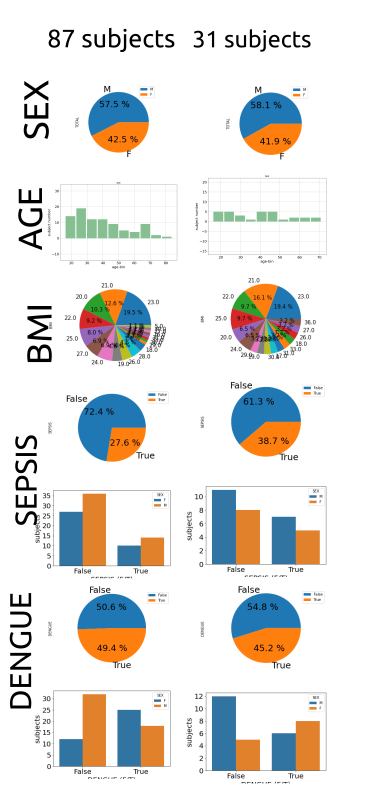
\includegraphics[width=\columnwidth]{../figures/patient-demographics-and-diseases/versions/drawing-v01}}%%GITHUB
    % {\includegraphics[width=\columnwidth]{figures/patient-demographics-and-diseases.png}}%%OVERLEAF
    %{\includegraphics[width=\columnwidth]{fig01.png}} %%ARXIV
\end{figure}

\section{Heuristics of model selection} \label{apd:heuristics}
\figureref{fig:ThinnerNeuralNetsResults} illustratres heristics for accuraty, train, classification and elapse times of 5 and 31 subjects.
\begin{figure*}[ht]
\floatconts
  {fig:ThinnerNeuralNetsResults}
%  {\caption{Heuristics for 5 and 33 subjects with 10 frames per clip and 25 batch size of clips using SqueezeNet \citep{iandola2017squeezenet}.}}
  {\caption{
    Heuristics for 5 and 31 subjects with 1 frames per clip and 20 batch size of clips for
    MobileNetV1 \citep{2017-howared_CoRR_MobileNetV1}, MobileNetV2 \citep{Sandler_2018_CVPR_MobileNetV2}, and SqueezeNet \citep{iandola2017squeezenet} 733,580
    %and ShrapML \citep{boice2022-in-jimaging} 430,000
          }.
  }
  {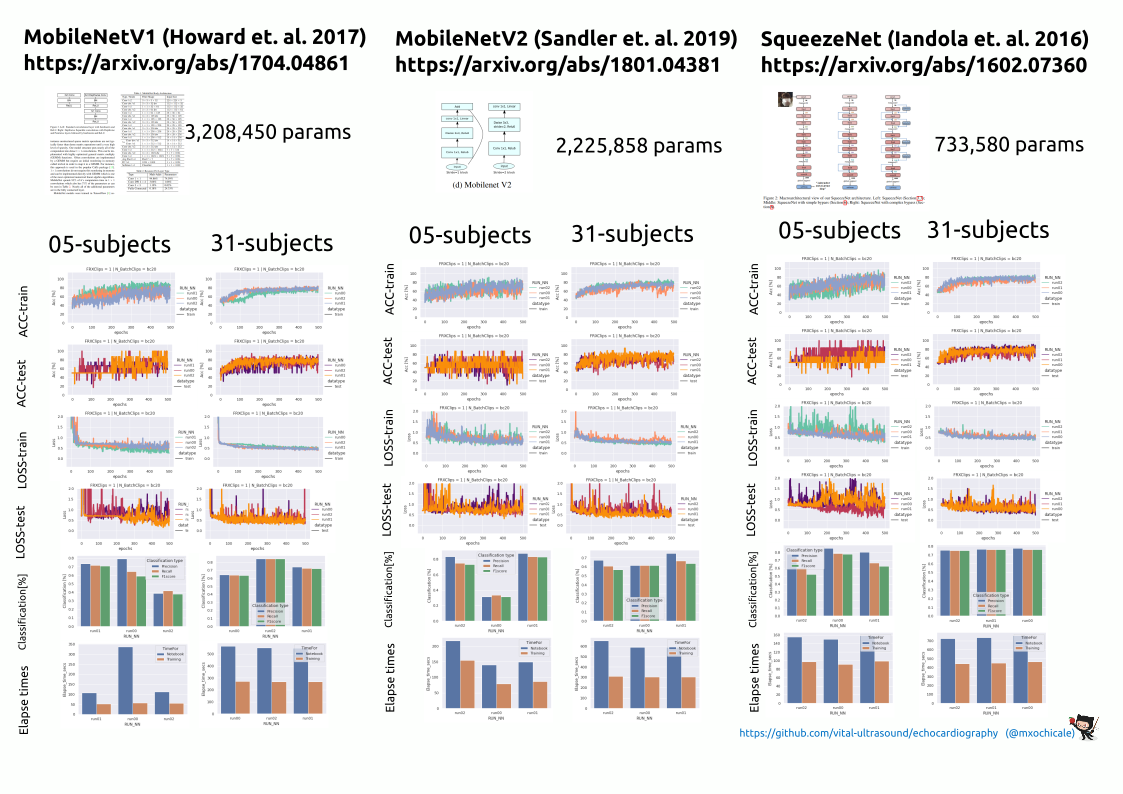
\includegraphics[width=\textwidth]{../figures/comparing-NETS-for-USviewclassification/versions/drawing-v00}}%%GITHUB
    % {\includegraphics[width=\columnwidth]{figures/squeezenet-05-33-subjects.png}}%%OVERLEAF
    %{\includegraphics[width=\columnwidth]{fig01.png}} %%ARXIV
\end{figure*}

\end{document}

%%%ARXIV

\newpage
\appendix

\section{Datasets}\label{apd:datasets}
\figureref{fig:demographics} illustrates demographics for sex, age, BMI, sepsis and denque for the complete dataset and the 31 subjects considered for this work.
\begin{figure}[htbp]
\floatconts
  {fig:demographics}
  {\caption{Patient demographics for sex, age, BMI, sepsis and dengue disease. Total number of patient is 87 of which data from 31 were curated, annotated and validated.}} %Figure is adapted from the works of %\cite{}.
  {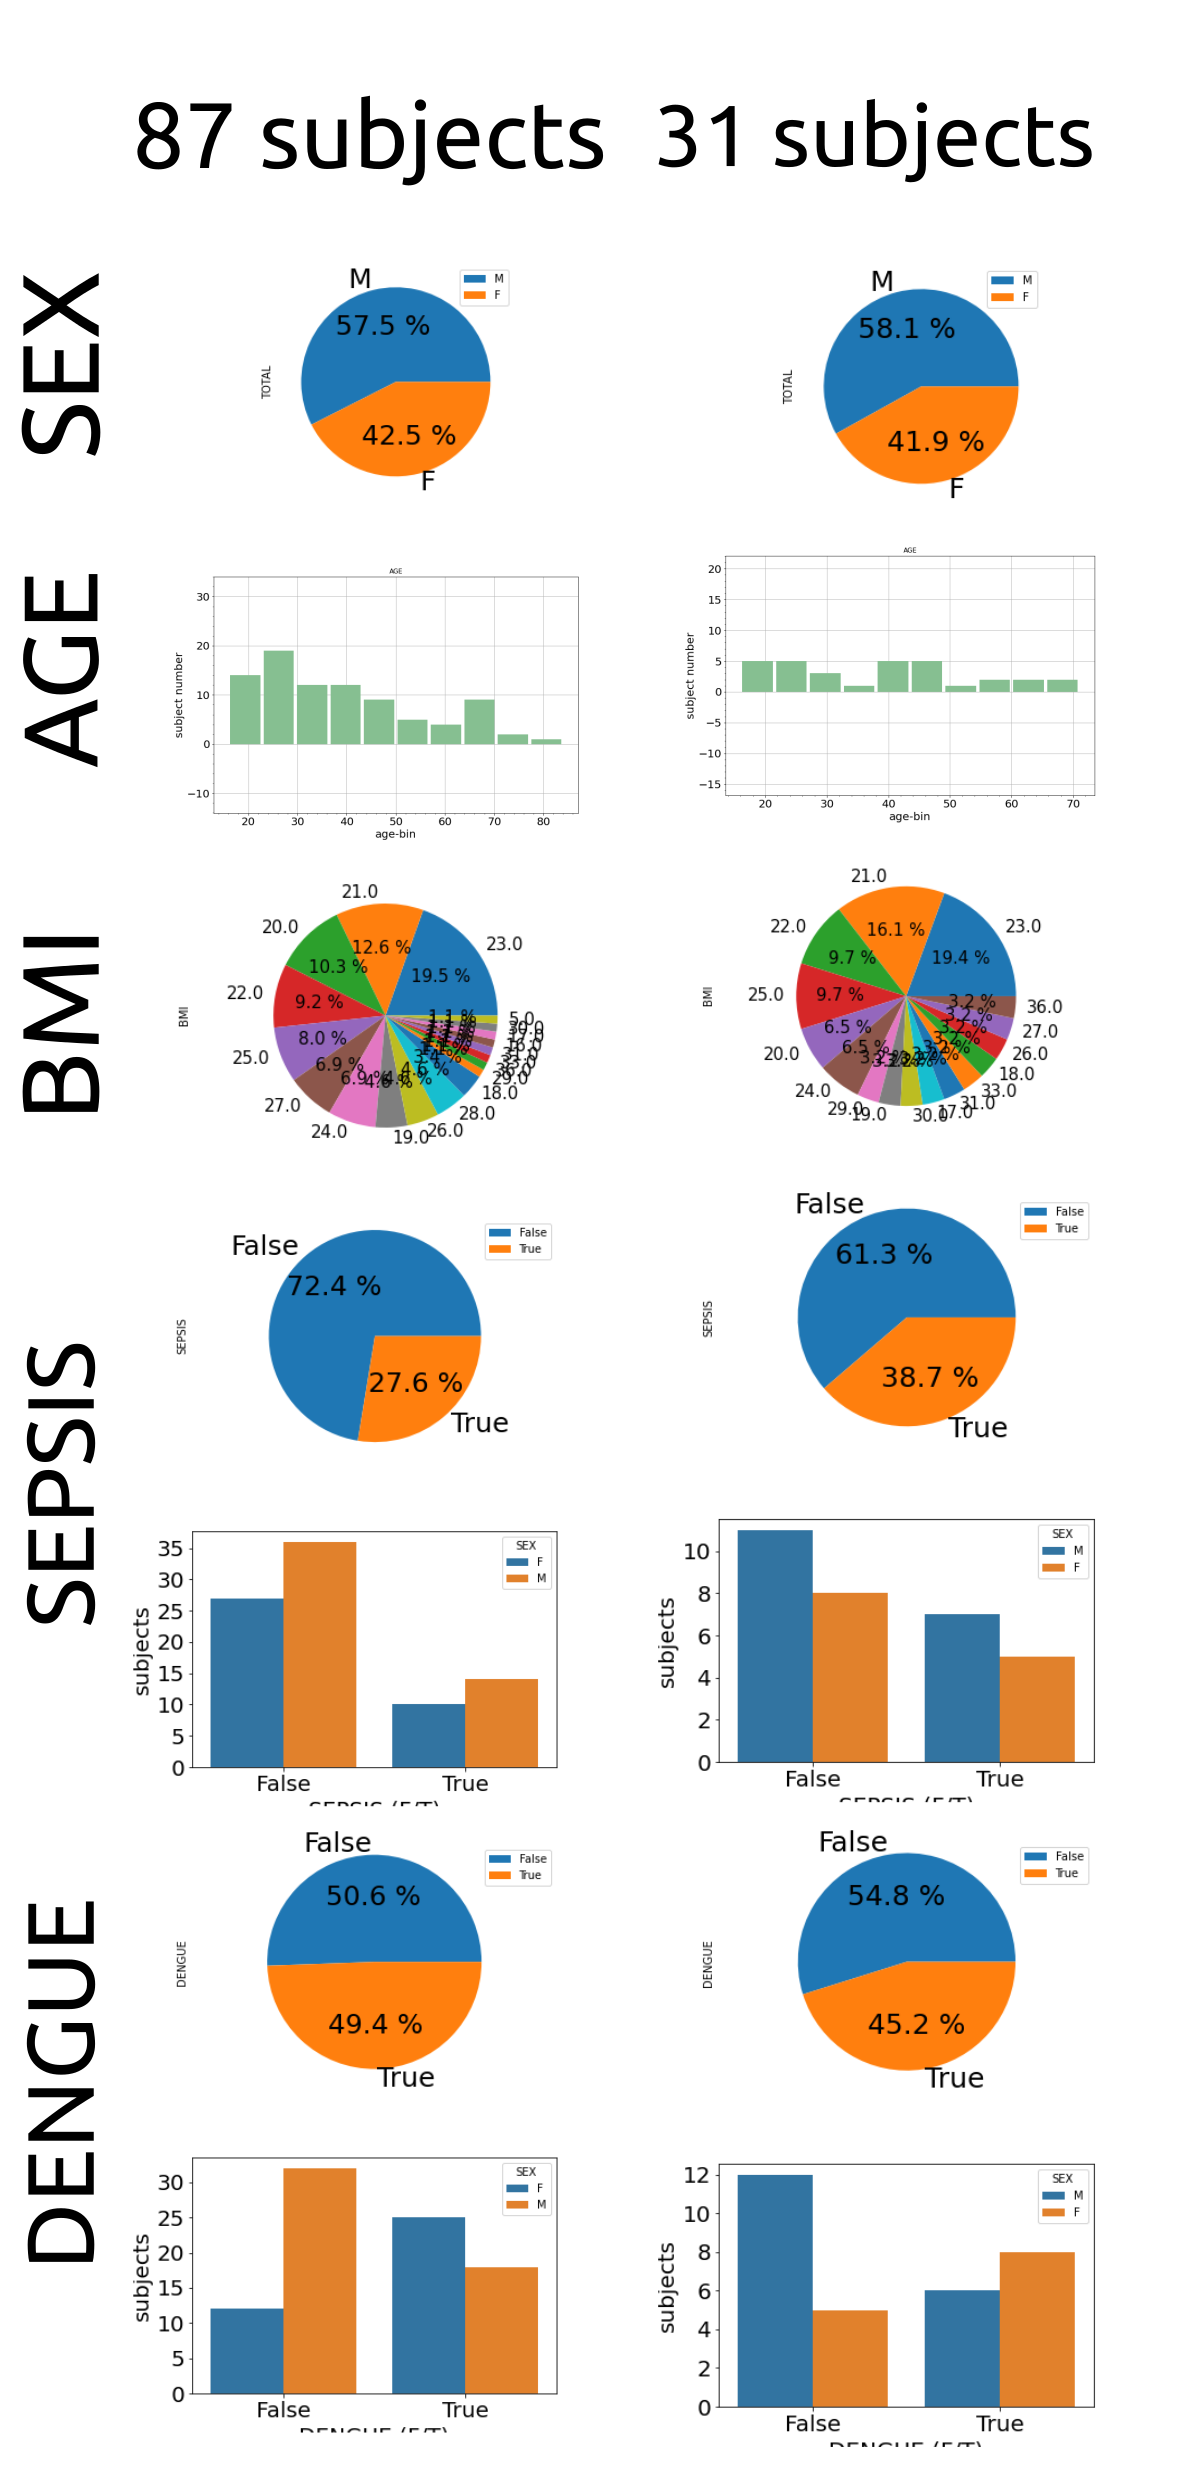
\includegraphics[width=\columnwidth]{../figures/patient-demographics-and-diseases/versions/drawing-v02}}%%GITHUB
    % {\includegraphics[width=\columnwidth]{figures/patient-demographics-and-diseases.png}}%%OVERLEAF
    %{\includegraphics[width=\columnwidth]{fig01.png}} %%ARXIV
\end{figure}

\section{Heuristics of model selection} \label{apd:heuristics}
\figureref{fig:ThinnerNeuralNetsResults} illustratres heristics for accuraty, train, classification and elapse times of 5 and 31 subjects.
\begin{figure*}[ht]
\floatconts
  {fig:ThinnerNeuralNetsResults}
%  {\caption{Heuristics for 5 and 33 subjects with 10 frames per clip and 25 batch size of clips using SqueezeNet \citep{iandola2017squeezenet}.}}
  {\caption{
    Heuristics for 5 and 31 subjects with 1 frames per clip and 20 batch size of clips for
    % VGG-based models~\citep{2015_Simonyan_ICLR}
    MobileNetV1~\citep{2017-howared_CoRR_MobileNetV1} with 3,208,450 parameters, MobileNetV2~\citep{Sandler_2018_CVPR_MobileNetV2} with 2,225,858 parameters, and SqueezeNet~\citep{iandola2017squeezenet} with 733,580 parameters
    %and ShrapML \citep{boice2022-in-jimaging} 430,000
          }.
  }
  {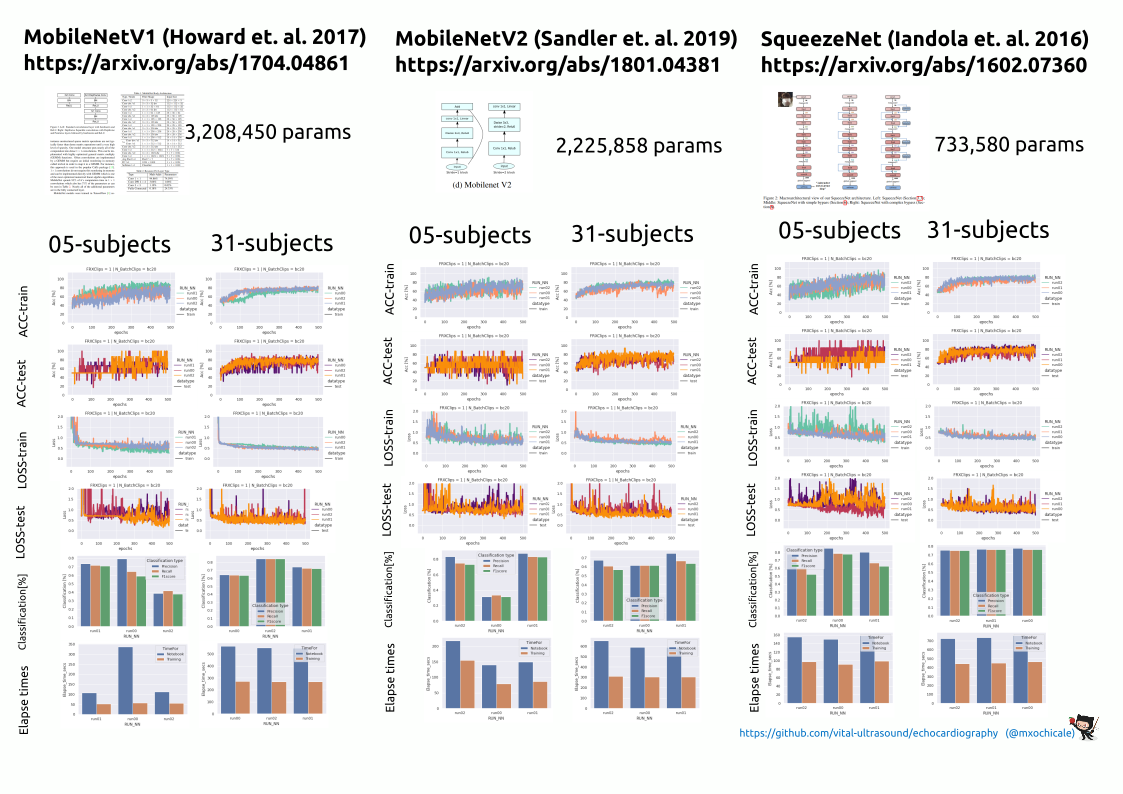
\includegraphics[width=\textwidth]{../figures/comparing-NETS-for-USviewclassification/versions/drawing-v00}}%%GITHUB
    % {\includegraphics[width=\columnwidth]{figures/squeezenet-05-33-subjects.png}}%%OVERLEAF
    %{\includegraphics[width=\columnwidth]{fig01.png}} %%ARXIV
\end{figure*}




\end{document}

